\documentclass{beamer}

\usepackage[utf8]{inputenc}
\usepackage{graphicx}
\graphicspath{ {./images/} }
\usetheme{Warsaw}
%\usecolortheme{beaver}

%Information to be included in the title page:
\title[Trayectorias ortogonales monocromáticas ajenas] %optional
{Trayectorias ortogonales monocromáticas ajenas}
\subtitle{}
\author[Rodrigo] % (optional, for multiple authors)
{C.~J.~Rodrigo~Guadalupe\inst{1}}
\institute[VFU] % (optional)
{
  \inst{1}%
  Instituto de Matemáticas\\
  Universidad Nacional Autónoma de México

}

\date[VNL 2020] % (optional)
{XXXV Coloquio Victor Neumann Lara, Marzo 2020}



\begin{document}

\frame{\titlepage}

\begin{frame}
\frametitle{Sample frame title}
This is a text in the first frame. This is a text in the first frame. This is a text in the first frame.
\end{frame}

\begin{frame}
 Aqui voy a poner las ideas principales de la plática \pause

texto \pause

Presentar una lo que es una L-linea, describir el problema, primero resolver parcialmente el problema con los arboles,i.e ,describir la construccion de las poligonos, ortognales, espirales, contruccion del arbol, decir porque se forma un arbol, pasar a la tranformacion de los 3 arboles a trayectorias, y mencionar el trabajo que despues se hizo (revisar las referencias del capitulo de libro de mikio kano)
\end{frame}
\begin{frame}
\begin{figure}[h]
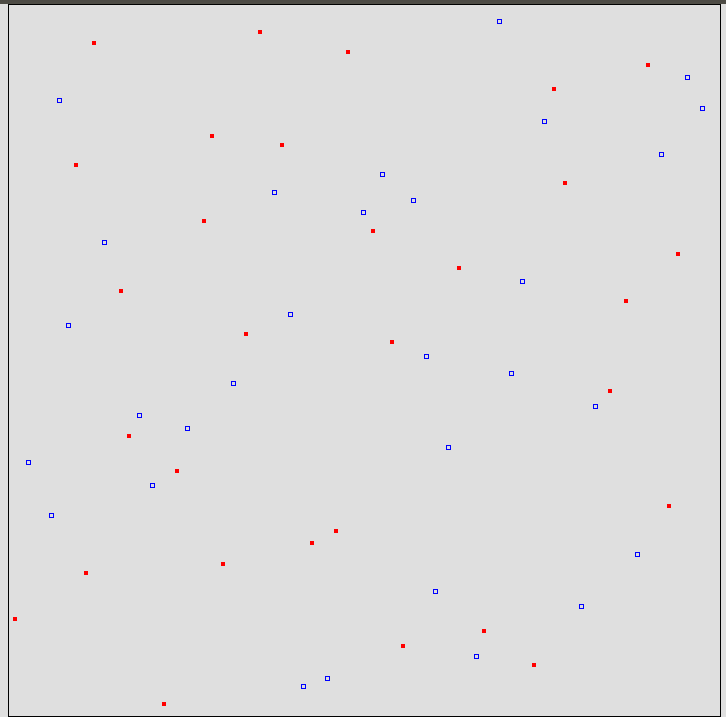
\includegraphics[width=6cm, height=6cm]{n-puntos}
\end{figure}
\end{frame}
\begin{frame}
\begin{figure}[h]
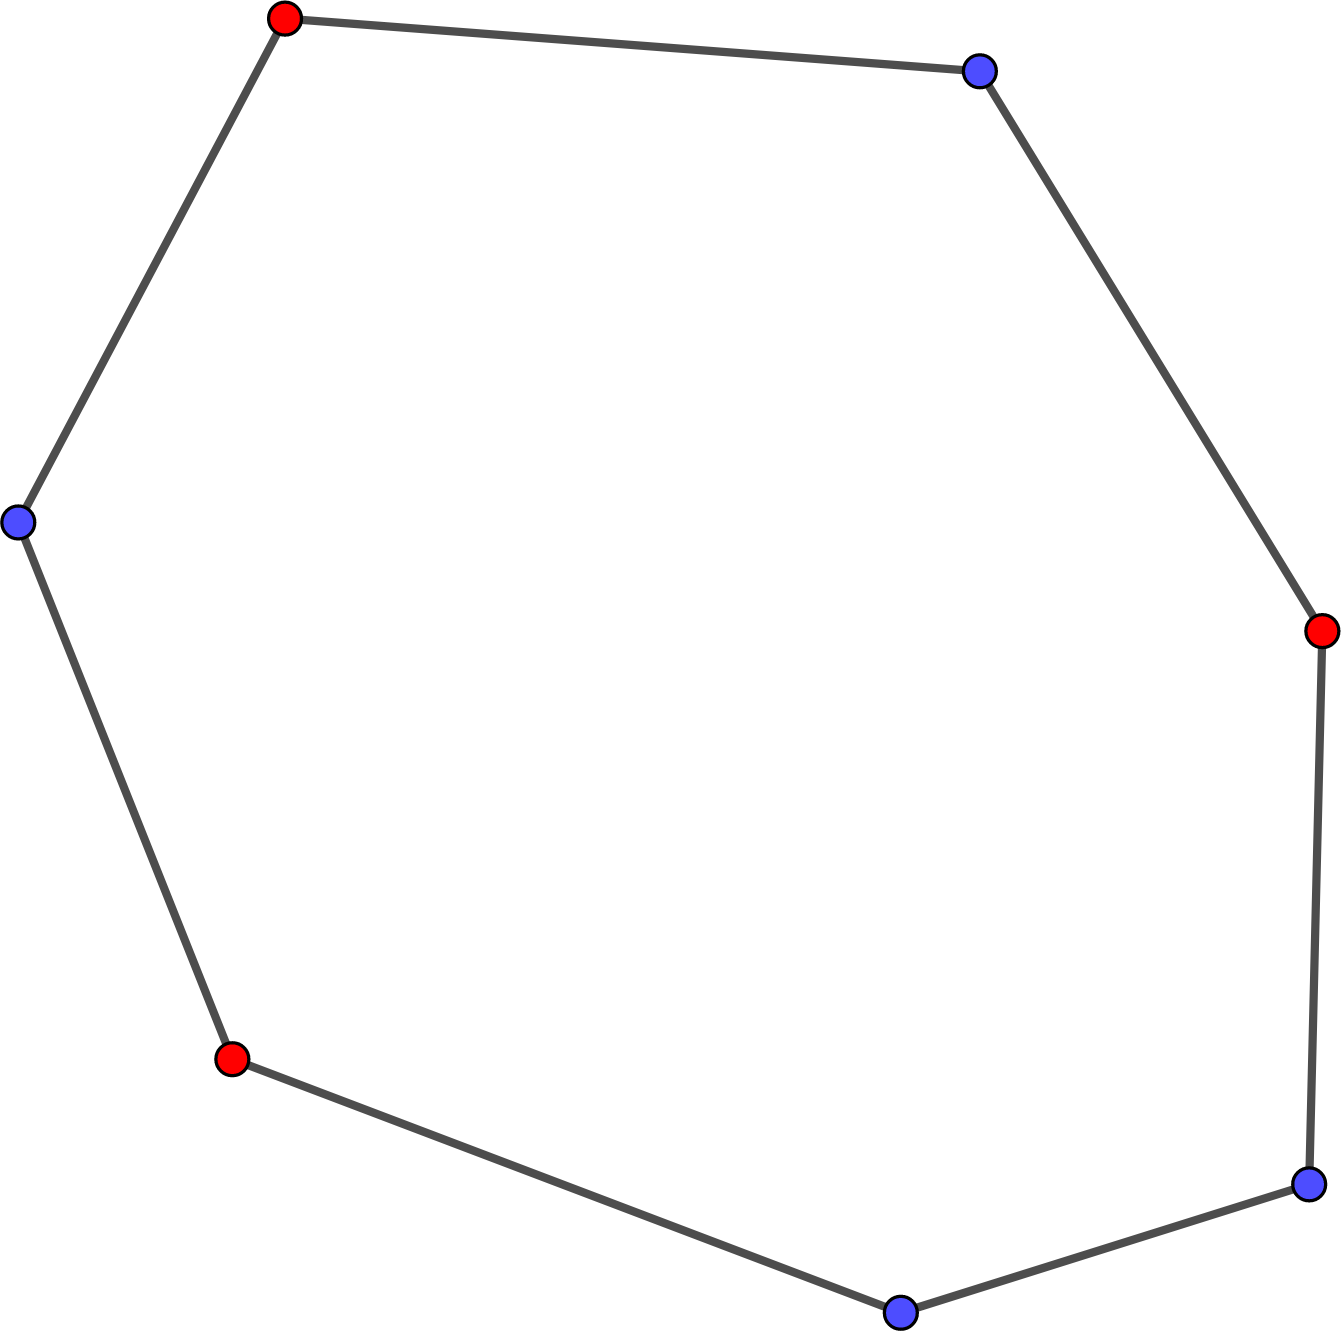
\includegraphics[width=\textwidth]{tauDeRyB}
\end{figure}
\end{frame}
\begin{frame}
Para un punto $x$ en el plano una linea en forma de $L$ consistente de dos rayos, uno vertical y otro horizontal emanentes de $x$ es llamado $L-linea$ con $esquina \, en \, x$
\end{frame}
\begin{frame}
\begin{figure}[h]
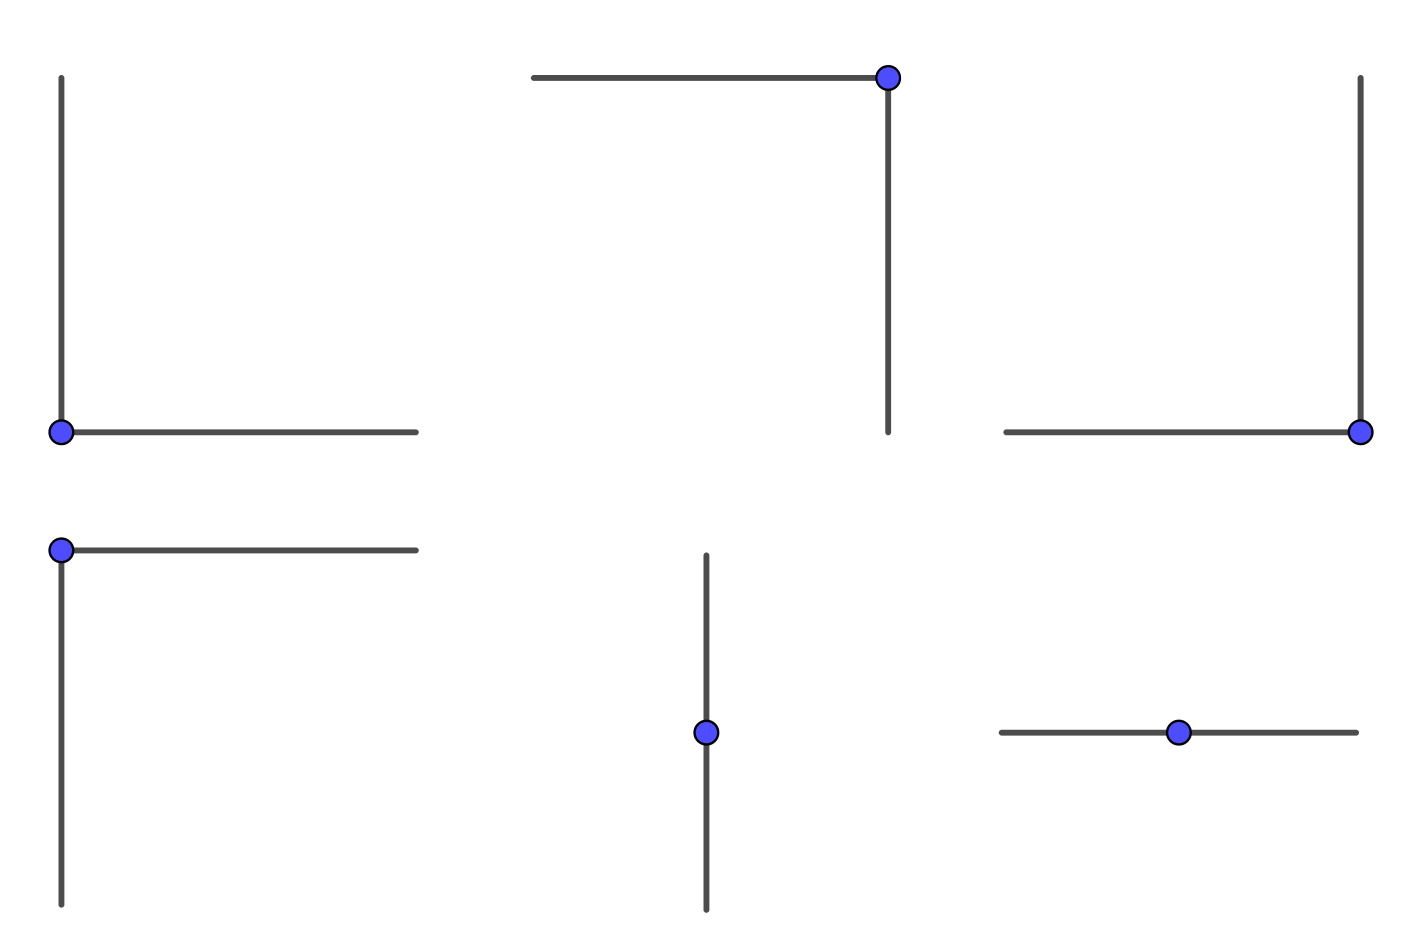
\includegraphics[width=\textwidth]{L-lineas}
\end{figure}
\end{frame}
\begin{frame}
\begin{figure}[h]
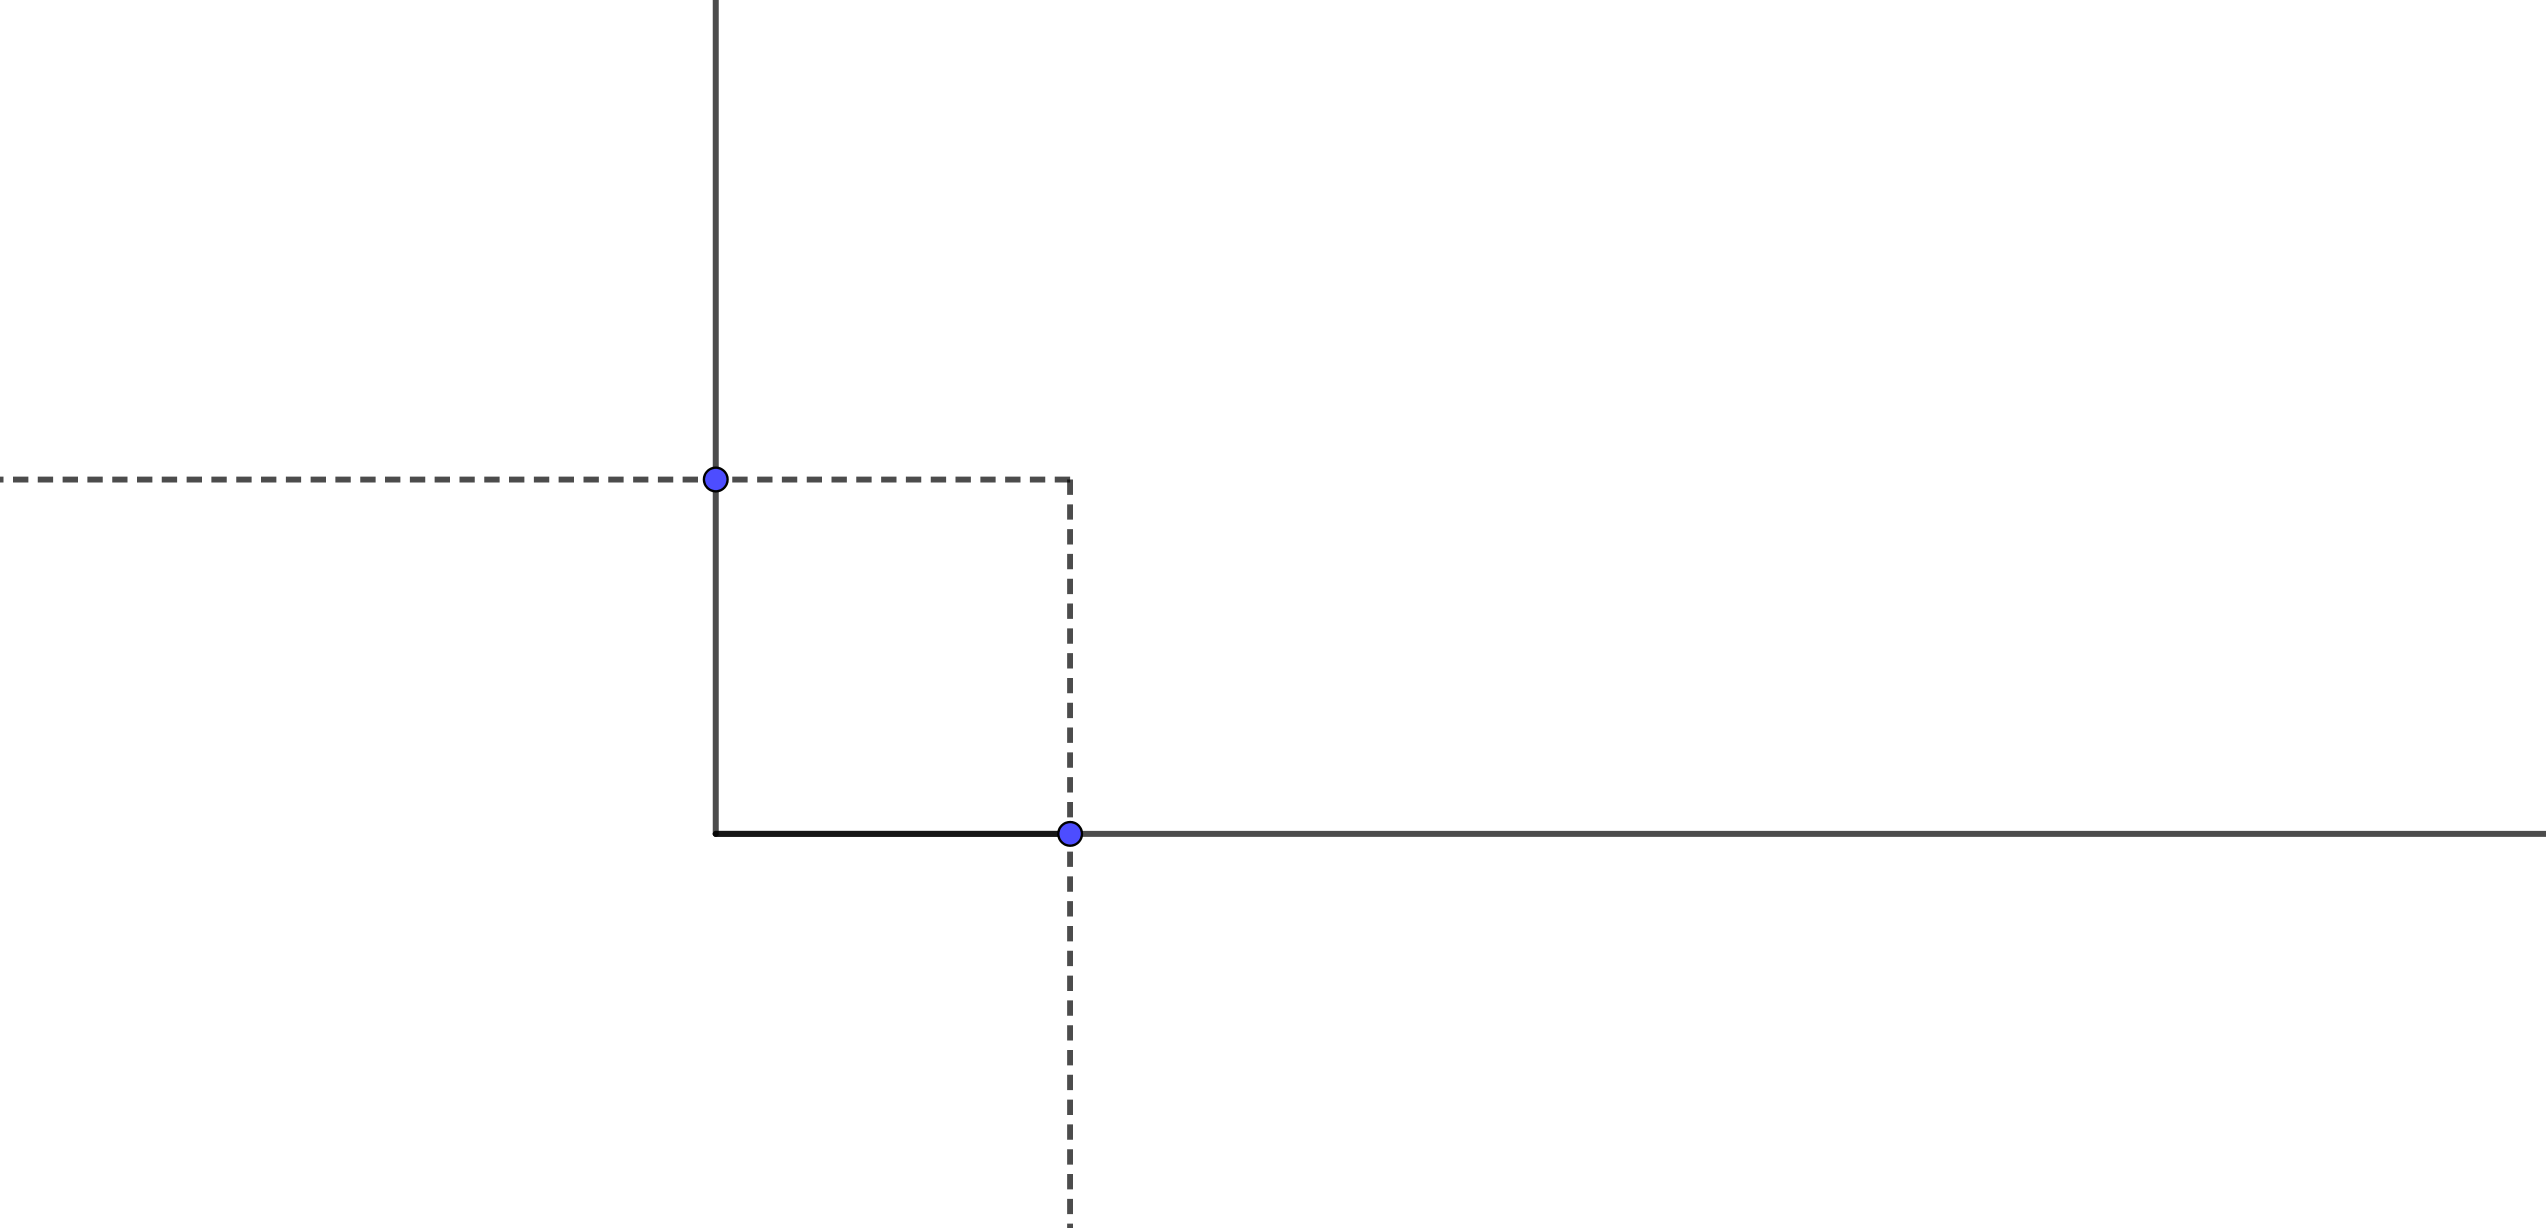
\includegraphics[width=\textwidth]{Diferencia-de-lineas-y-L-lineas}
\end{figure}
\end{frame}
\begin{frame}
\begin{figure}[h]
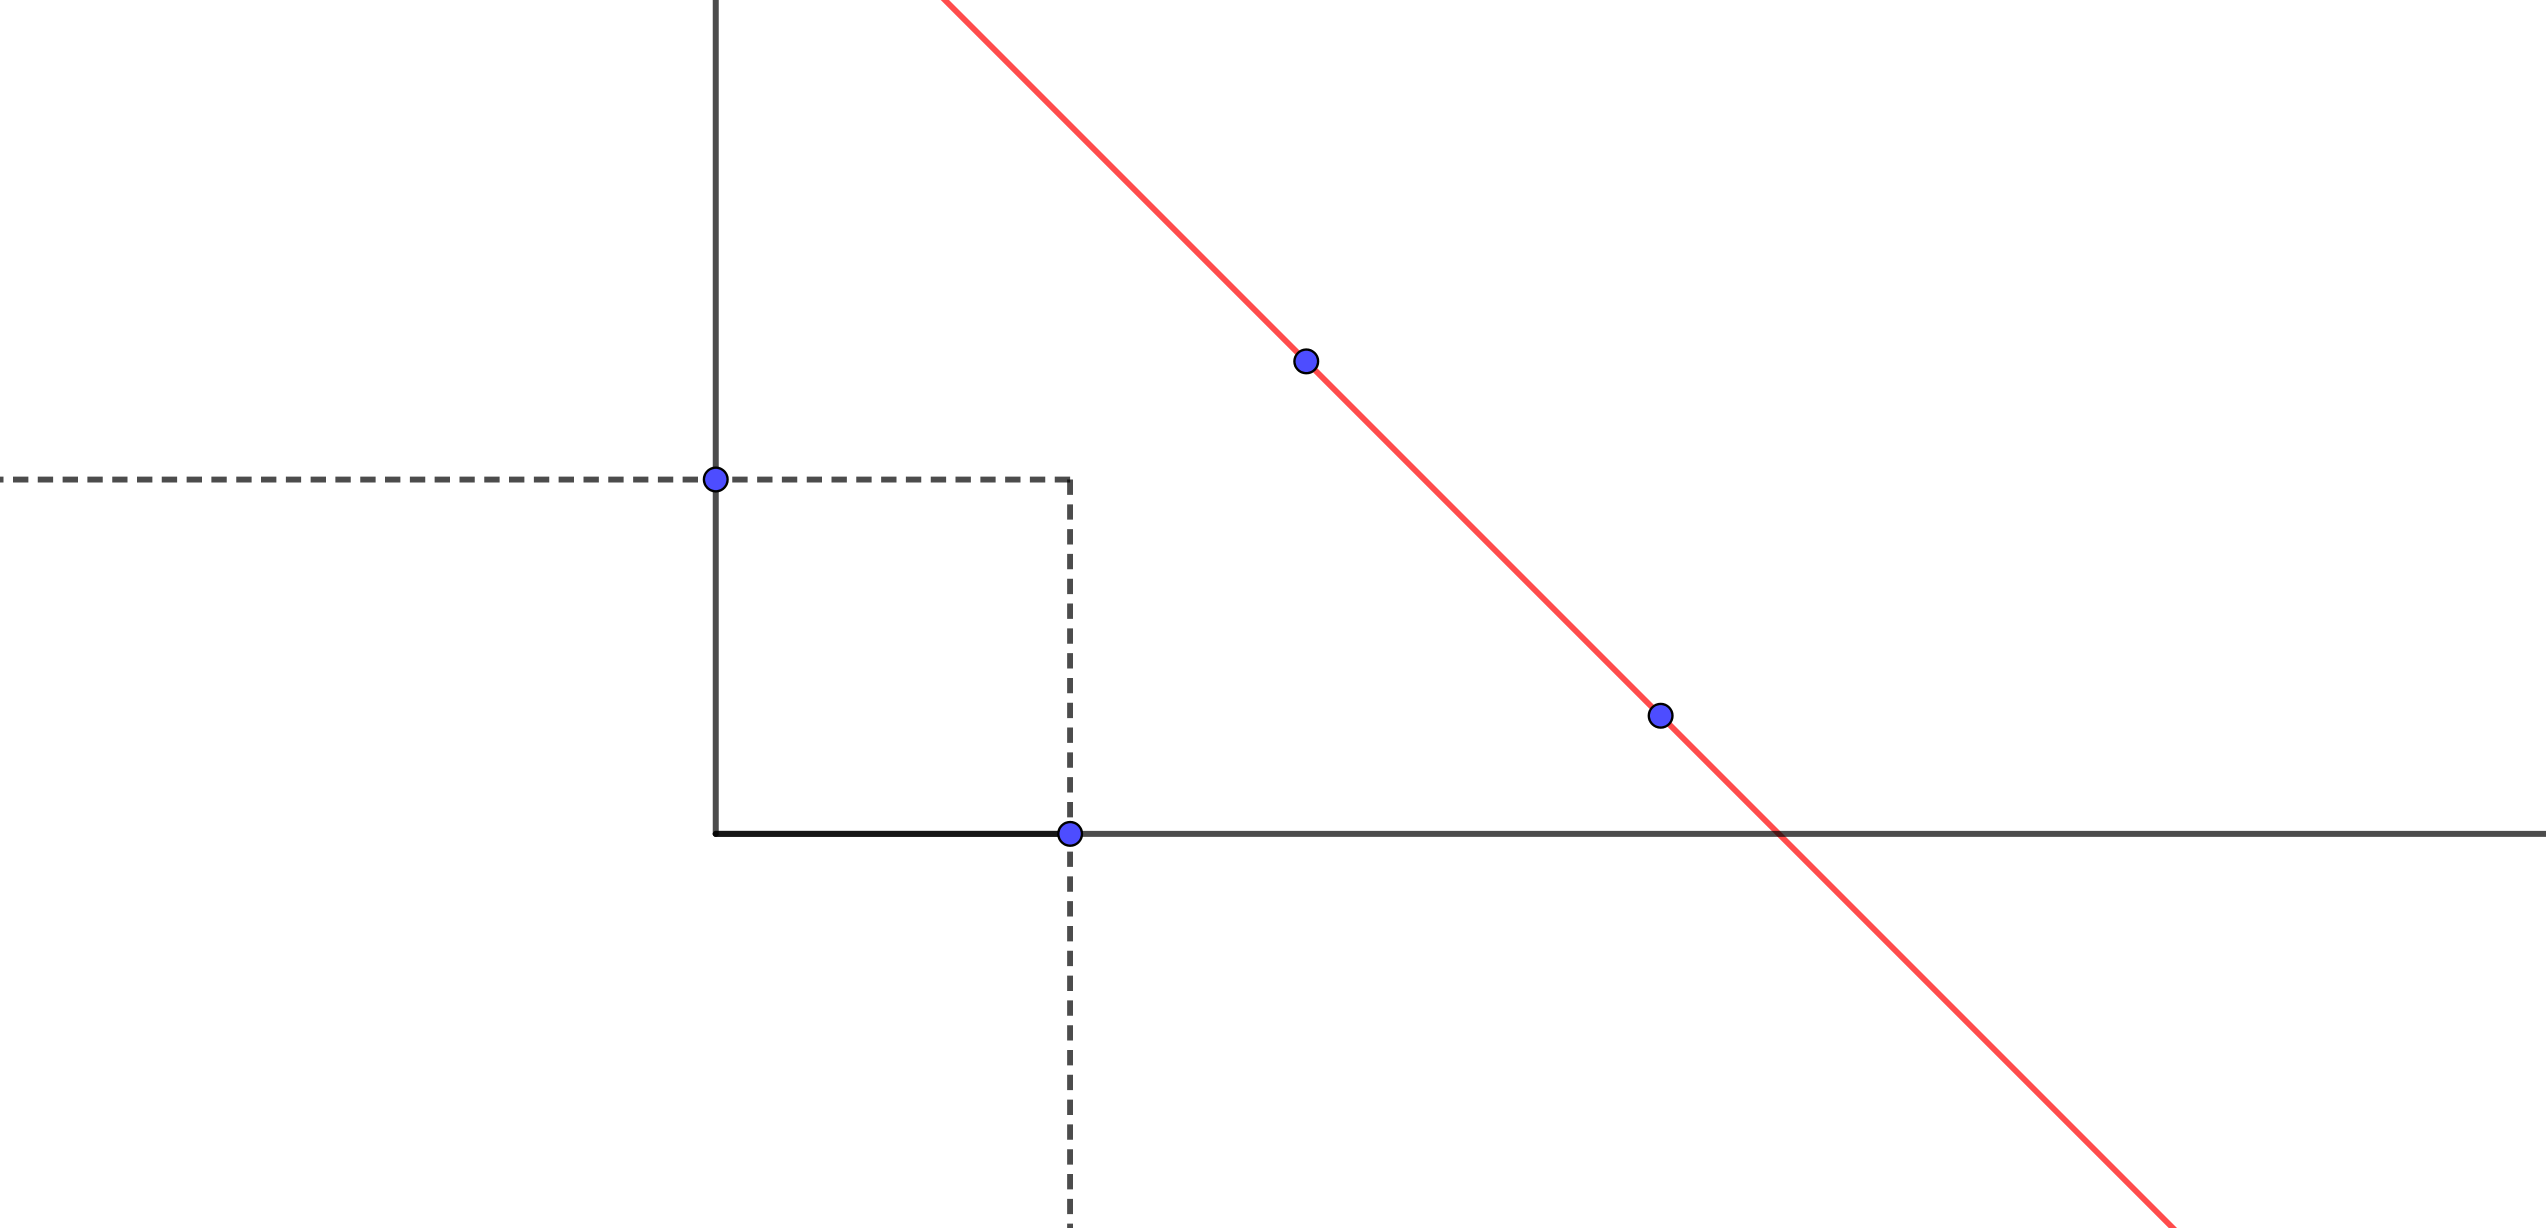
\includegraphics[width=\textwidth]{Diferencia-de-lineas-y-L-lineas-2}
\end{figure}
\end{frame}
\begin{frame}
\begin{figure}[h]
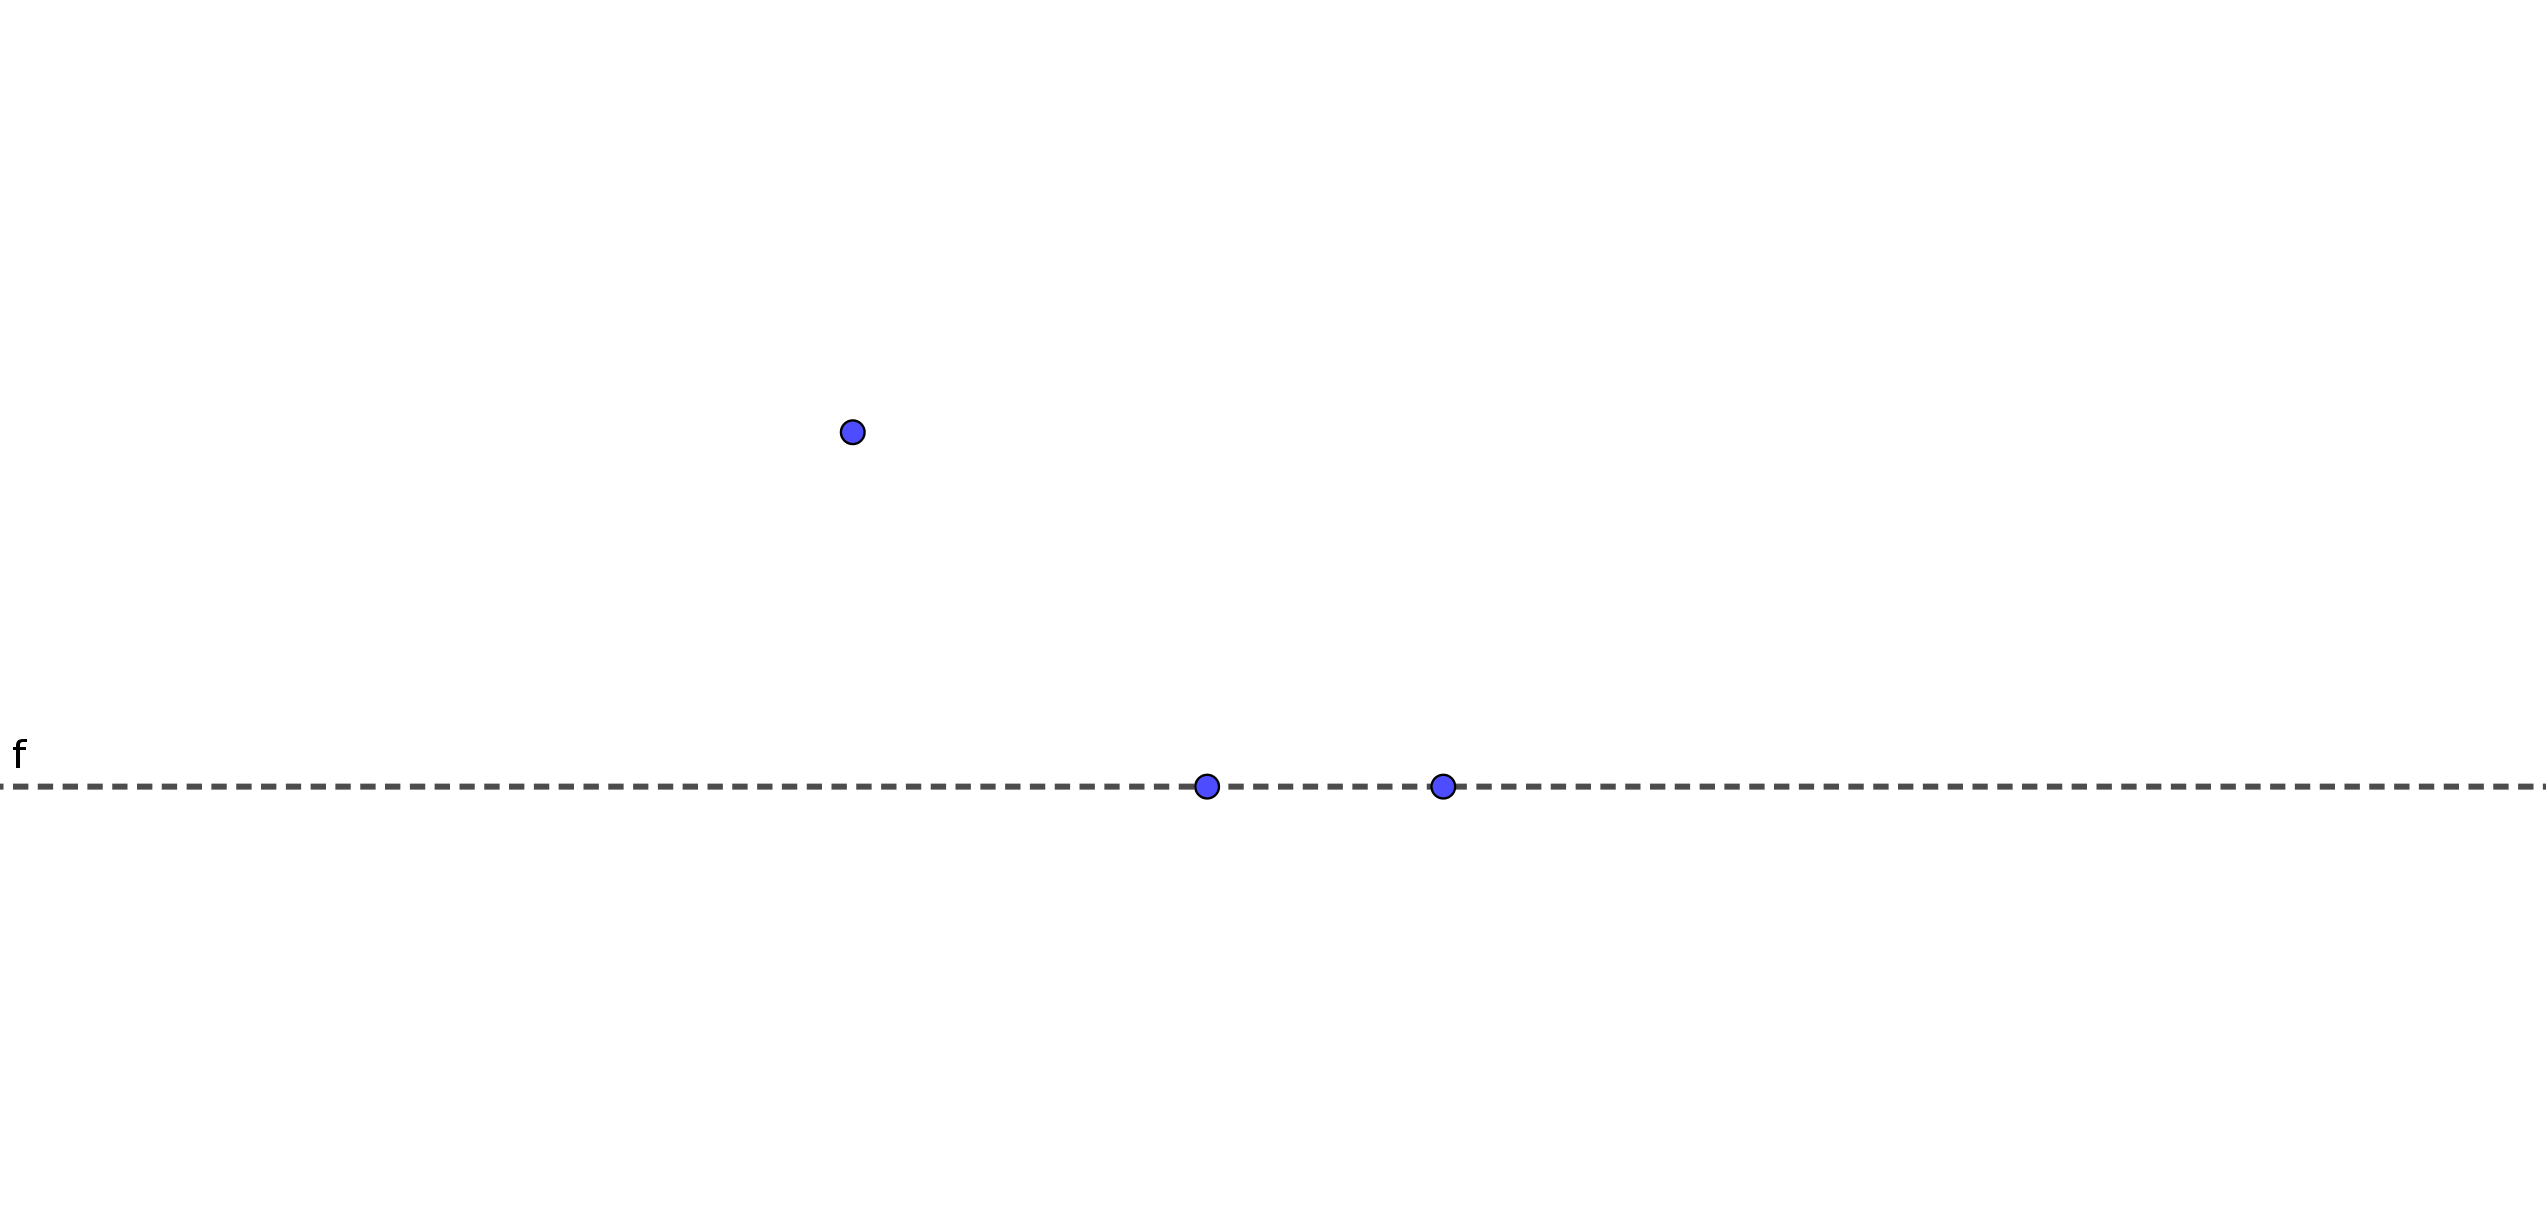
\includegraphics[width=\textwidth]{Posicion-general}
\end{figure}
\end{frame}
\begin{frame}
\begin{figure}[h]
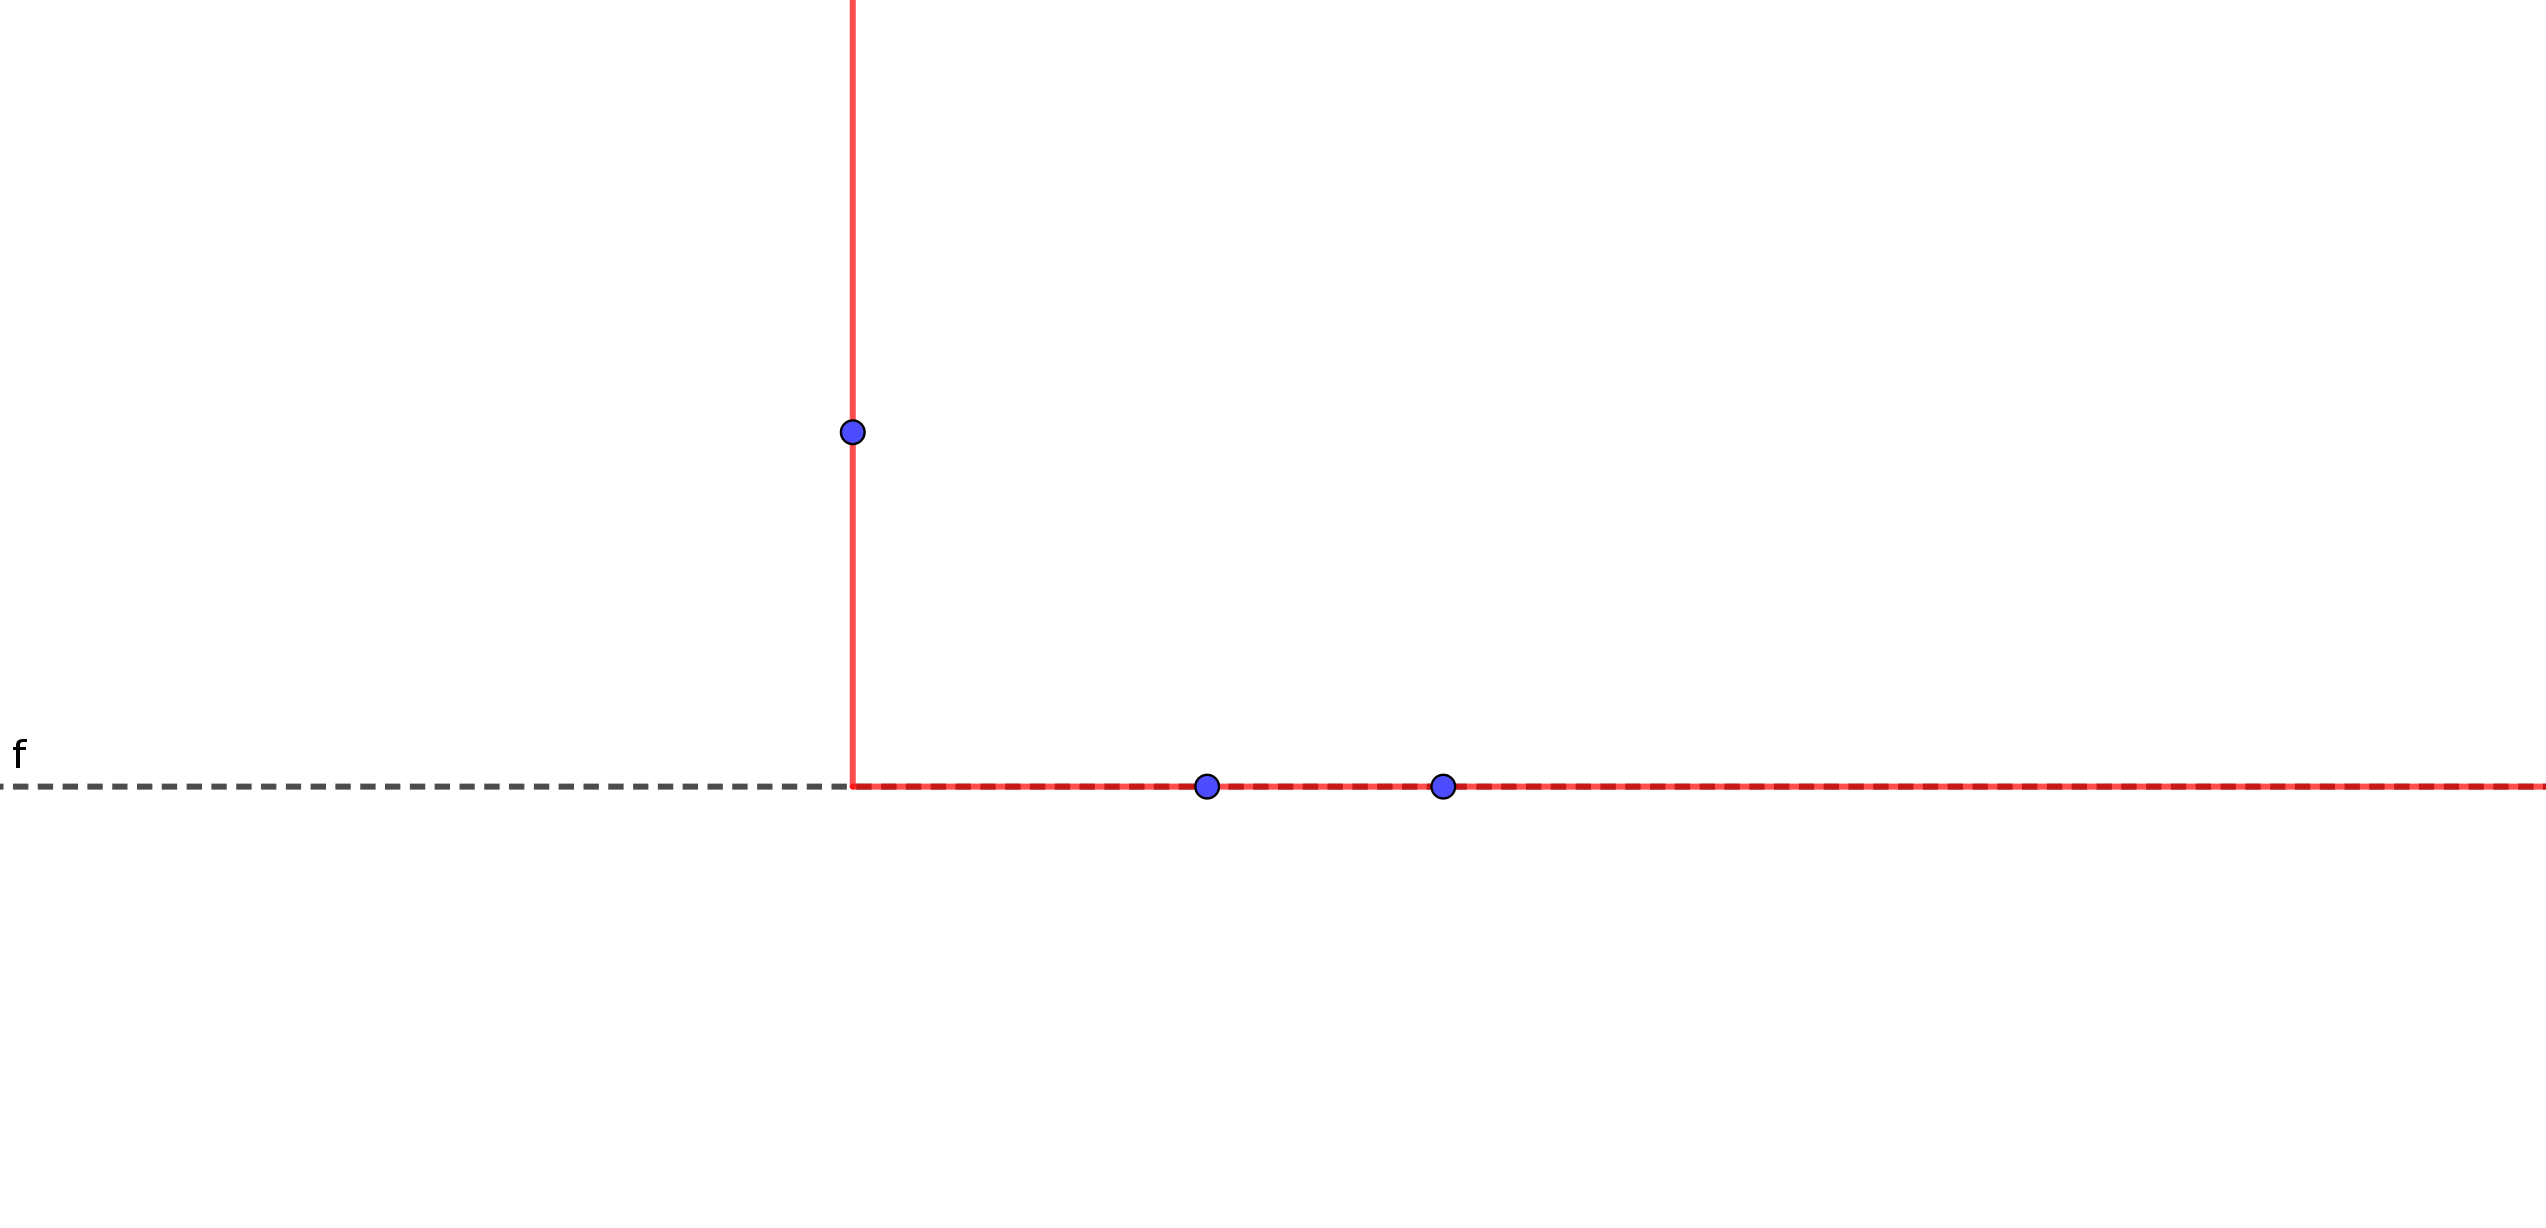
\includegraphics[width=\textwidth]{Posicion-general-2}
\end{figure}
\end{frame}
\begin{frame}
\begin{figure}[h]
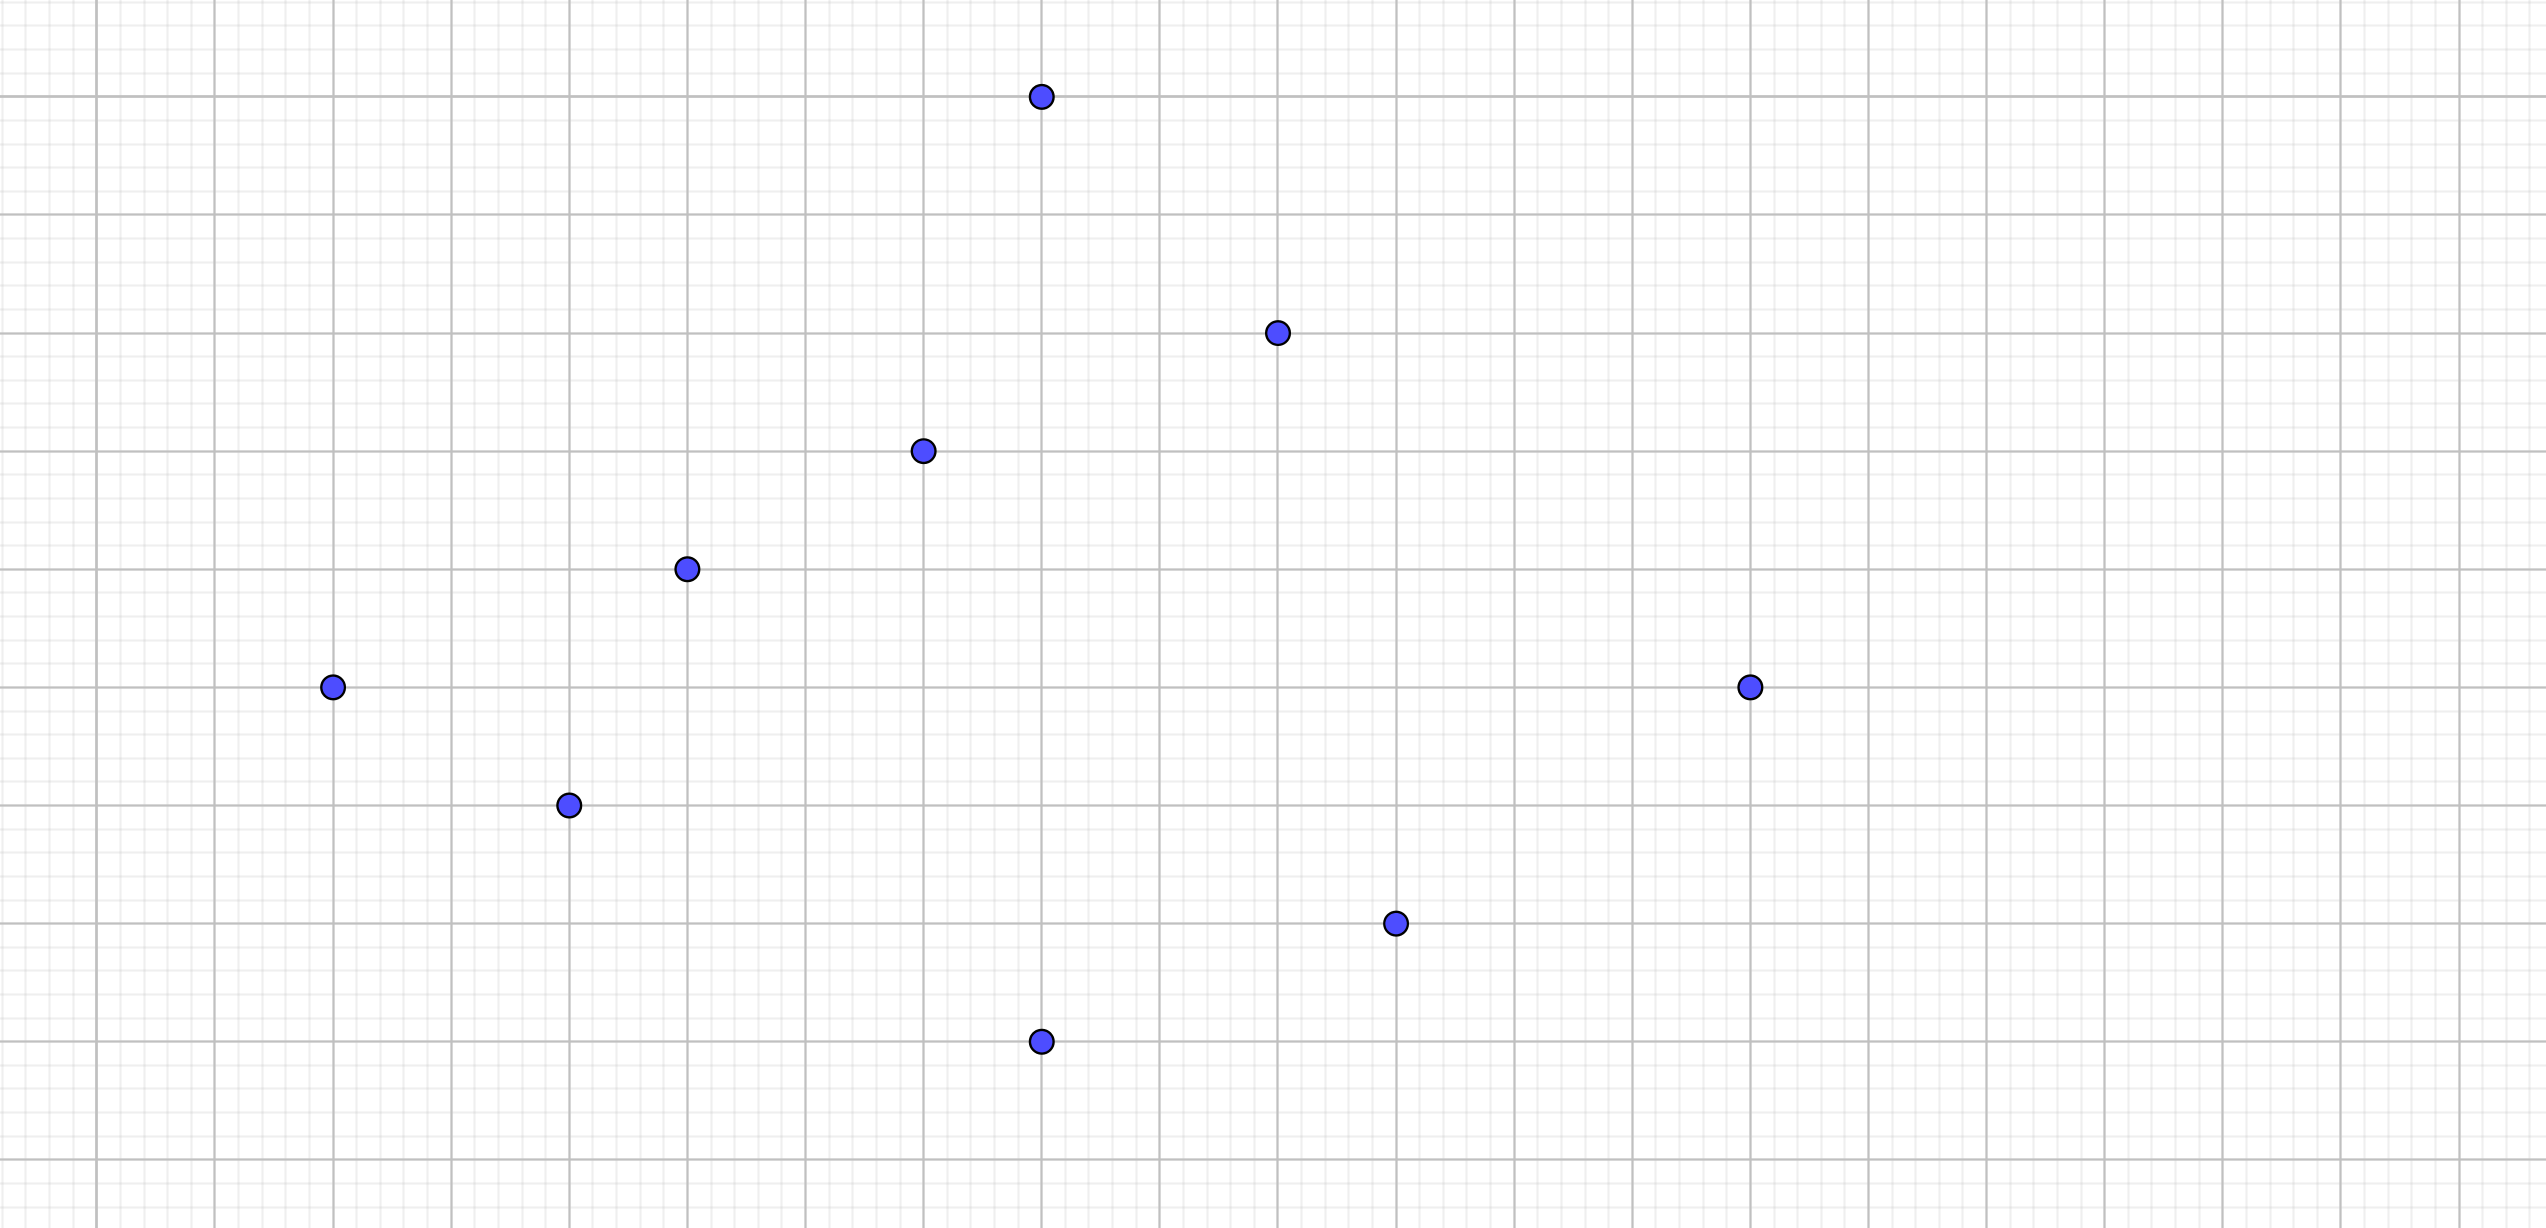
\includegraphics[width=\textwidth]{Prueba-misma-vertical}
\end{figure}
\end{frame}
\begin{frame}
\begin{figure}[h]
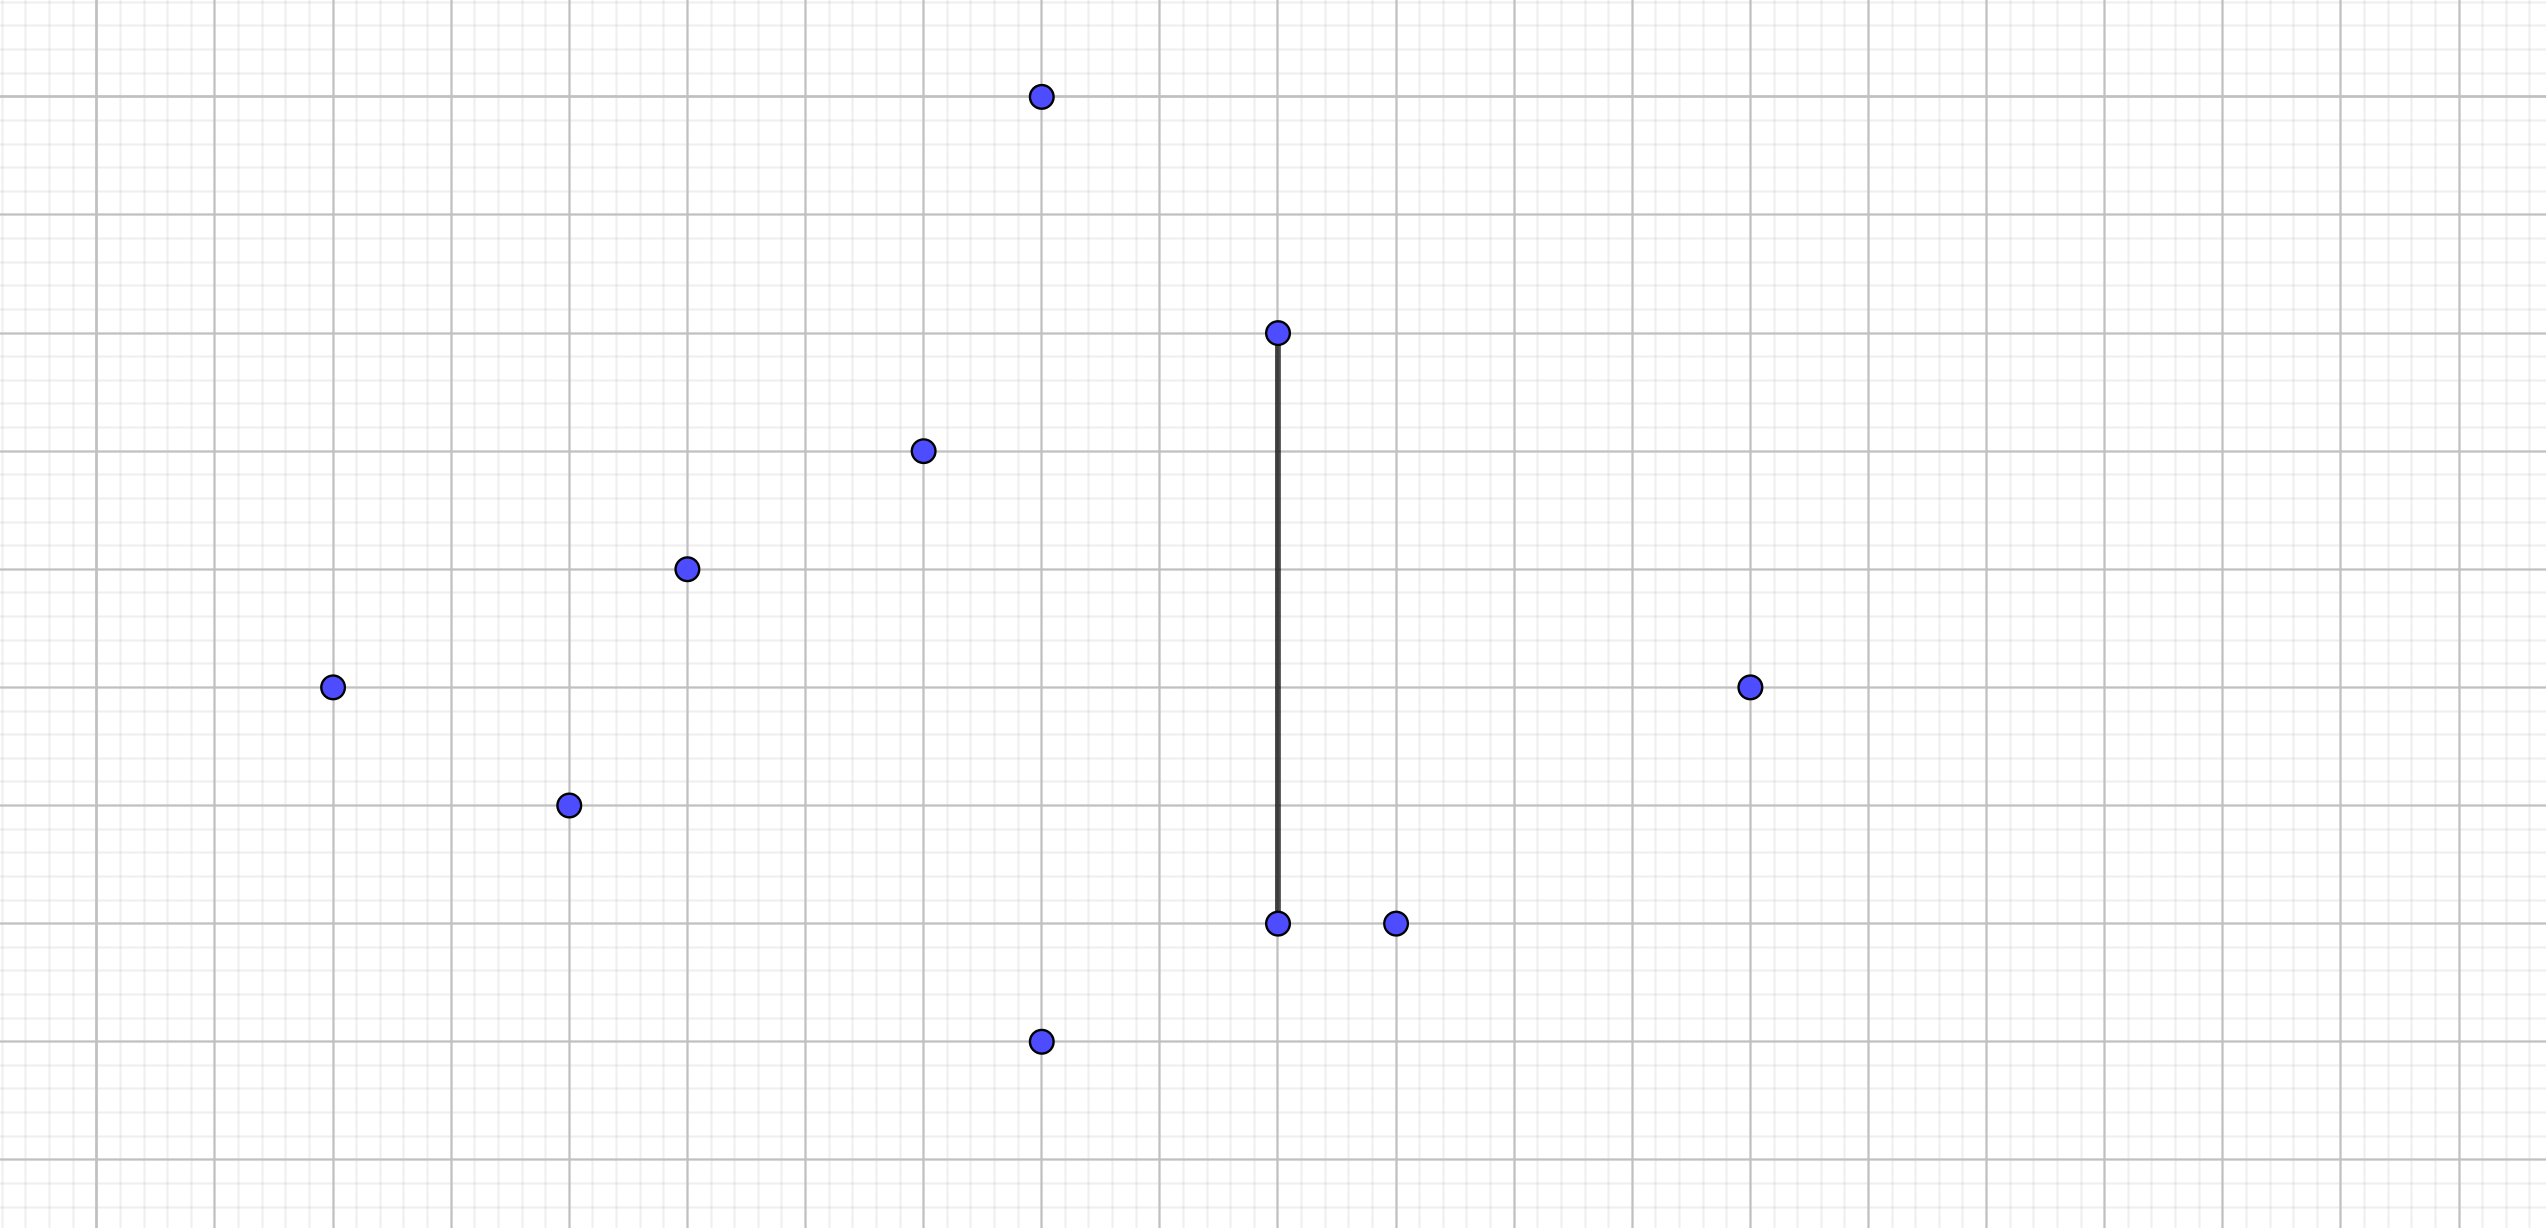
\includegraphics[width=\textwidth]{Prueba-misma-vertical-2}
\end{figure}
\end{frame}
\begin{frame}
\begin{figure}[h]
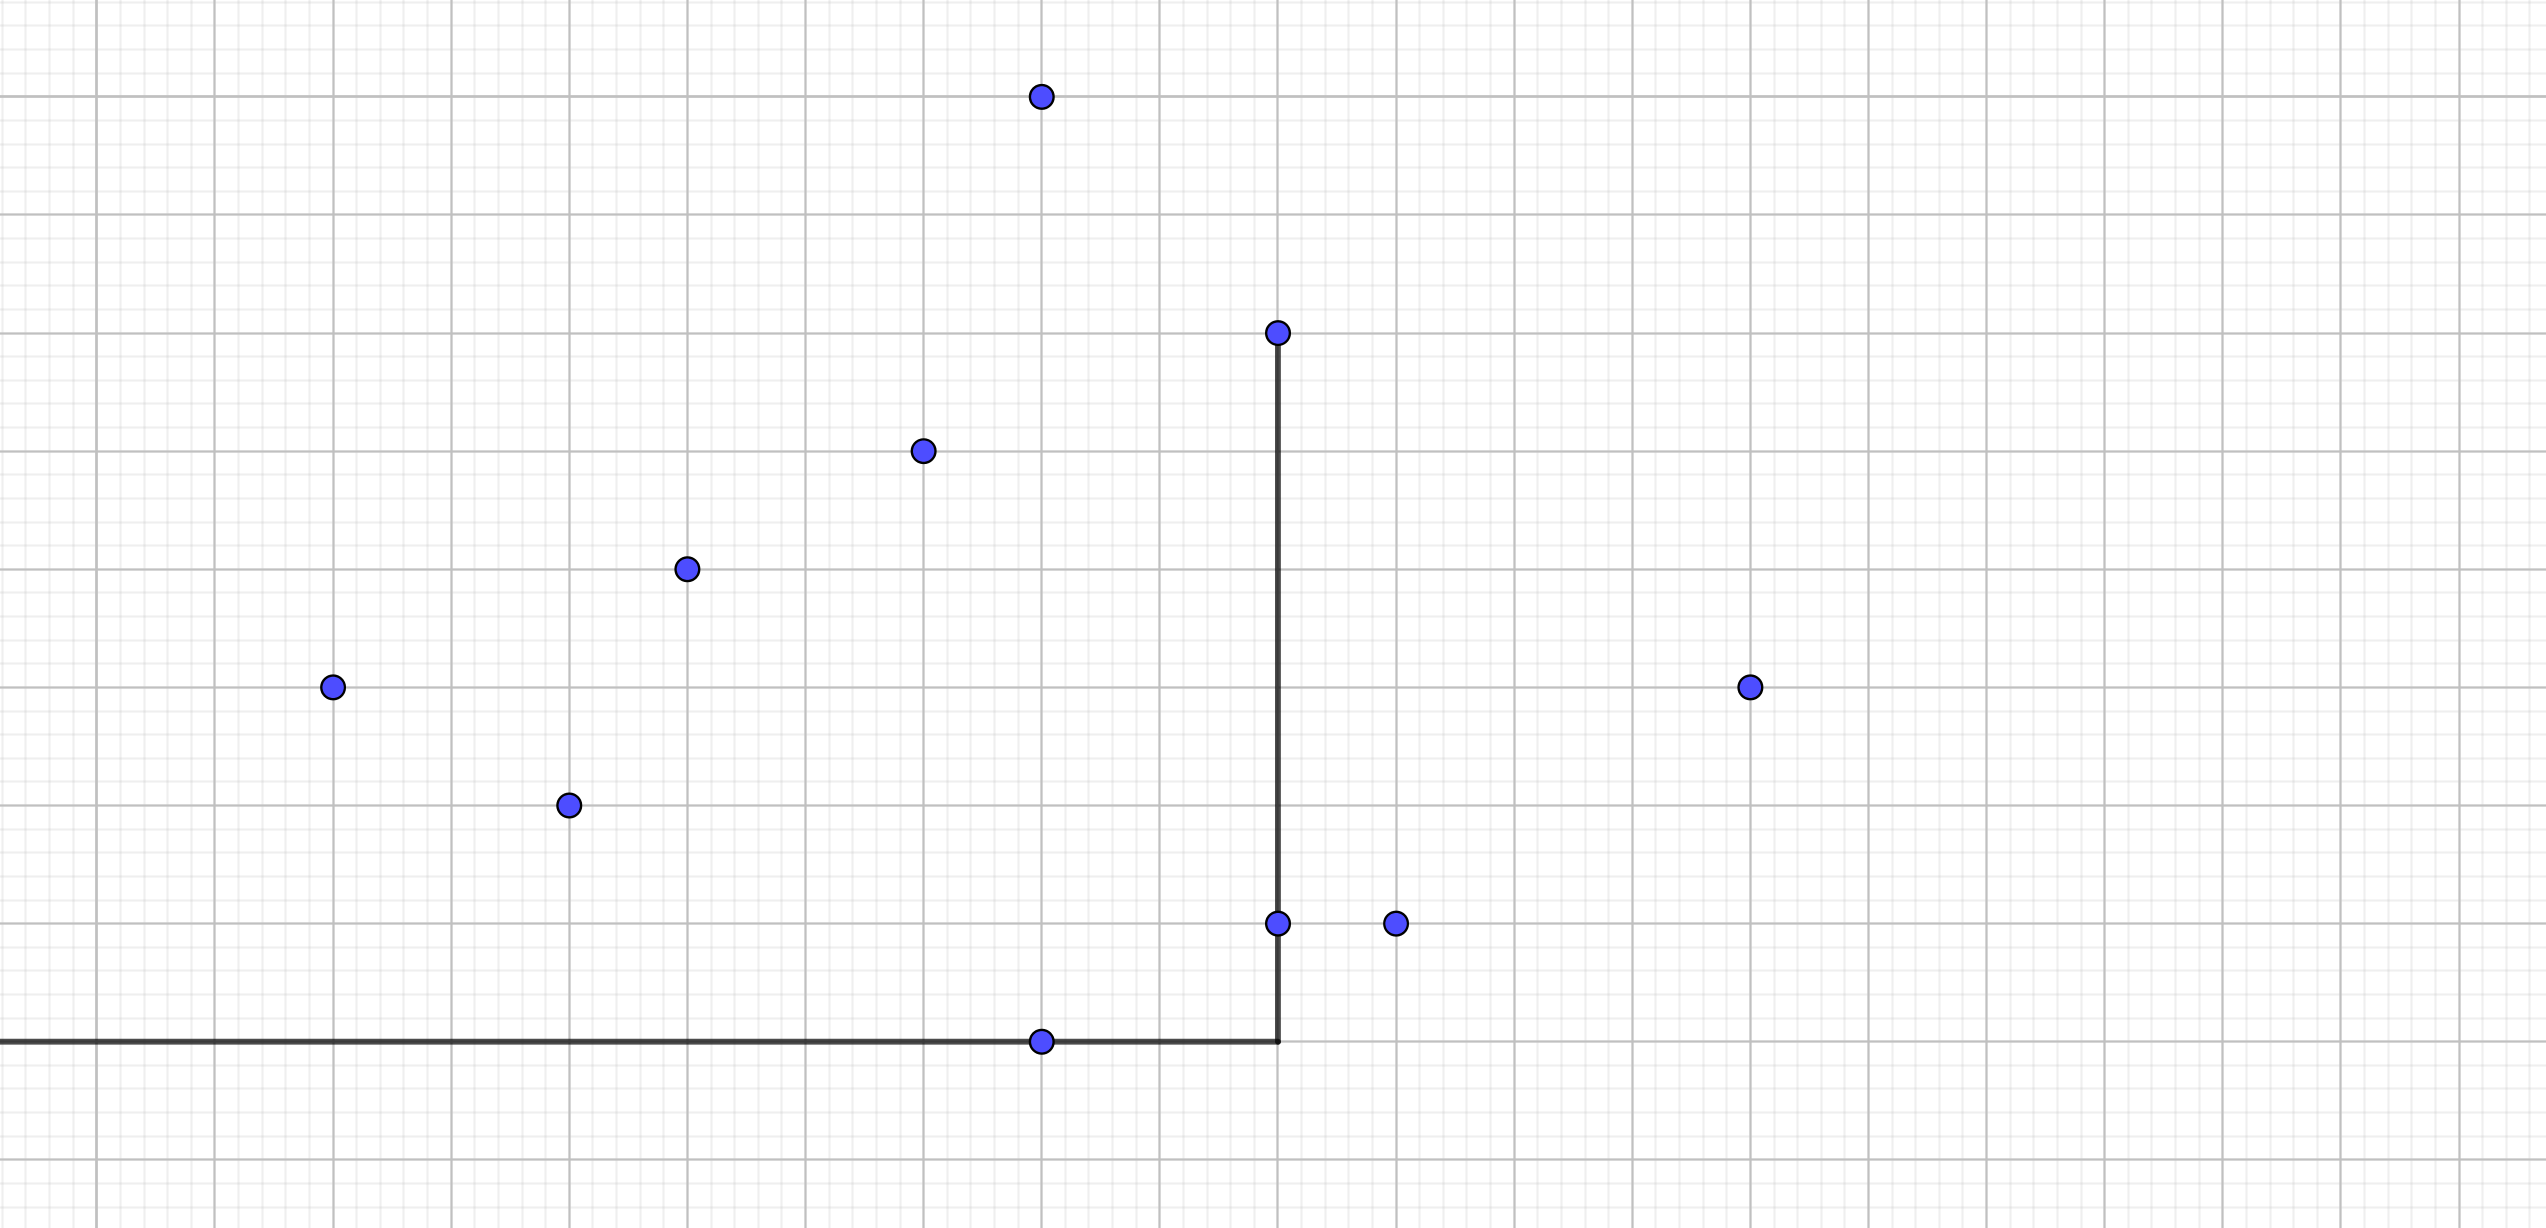
\includegraphics[width=\textwidth]{Prueba-misma-vertical-3}
\end{figure}
\end{frame}
\begin{frame}
\begin{figure}[h]
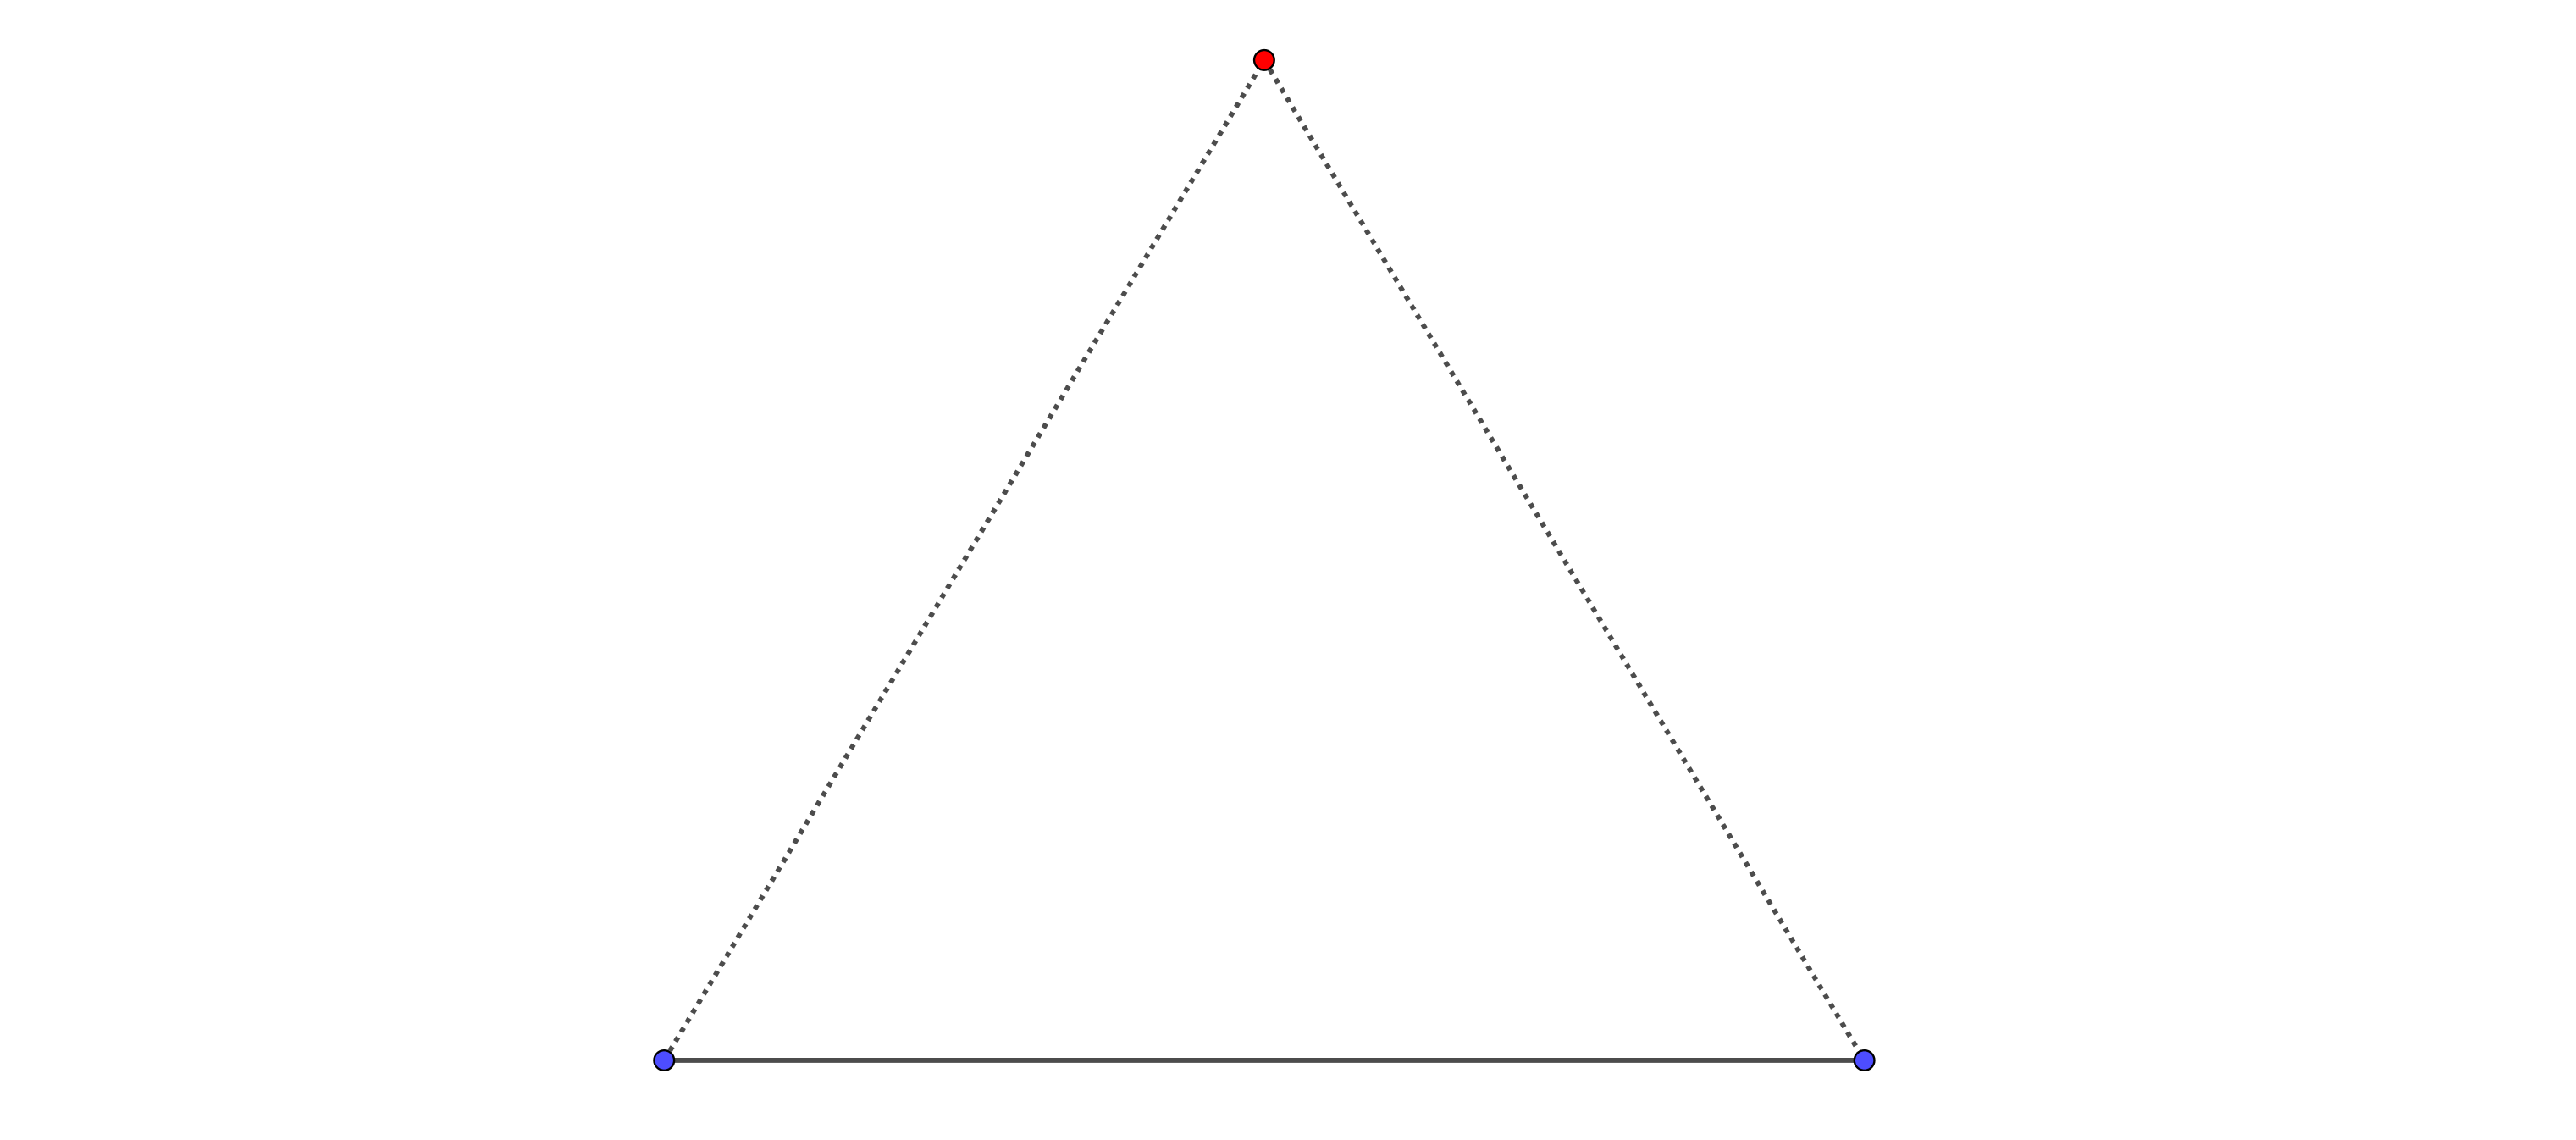
\includegraphics[width=\textwidth]{Tokunaga}
\end{figure}
\end{frame}
\begin{frame}
\begin{figure}[h]
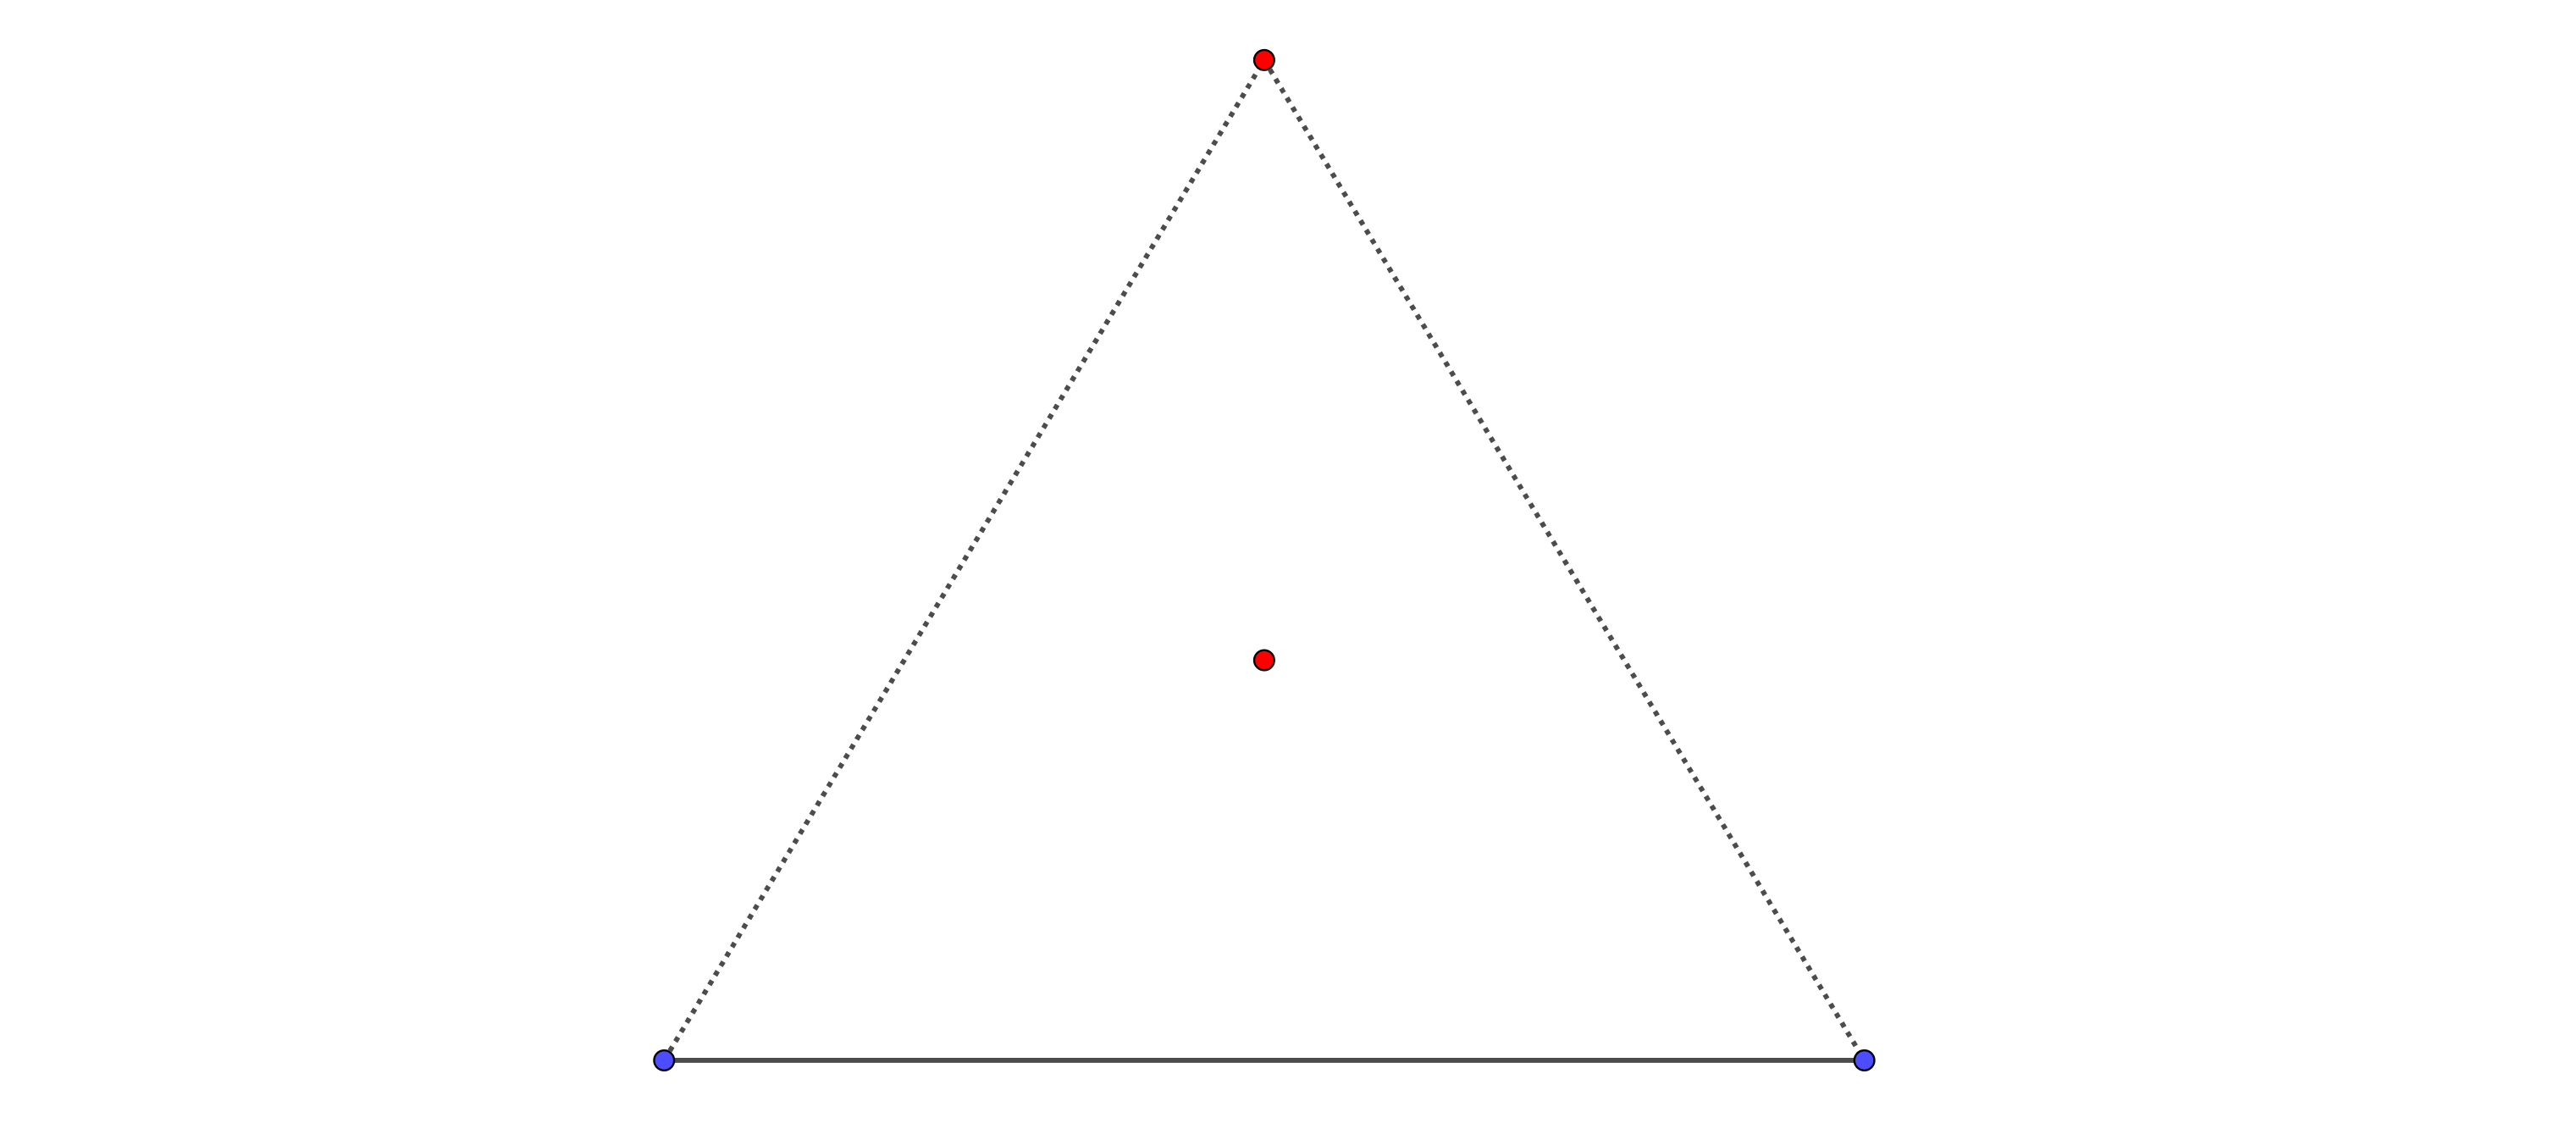
\includegraphics[width=\textwidth]{Tokunaga-2}
\end{figure}
\end{frame}
\begin{frame}
\begin{figure}[h]
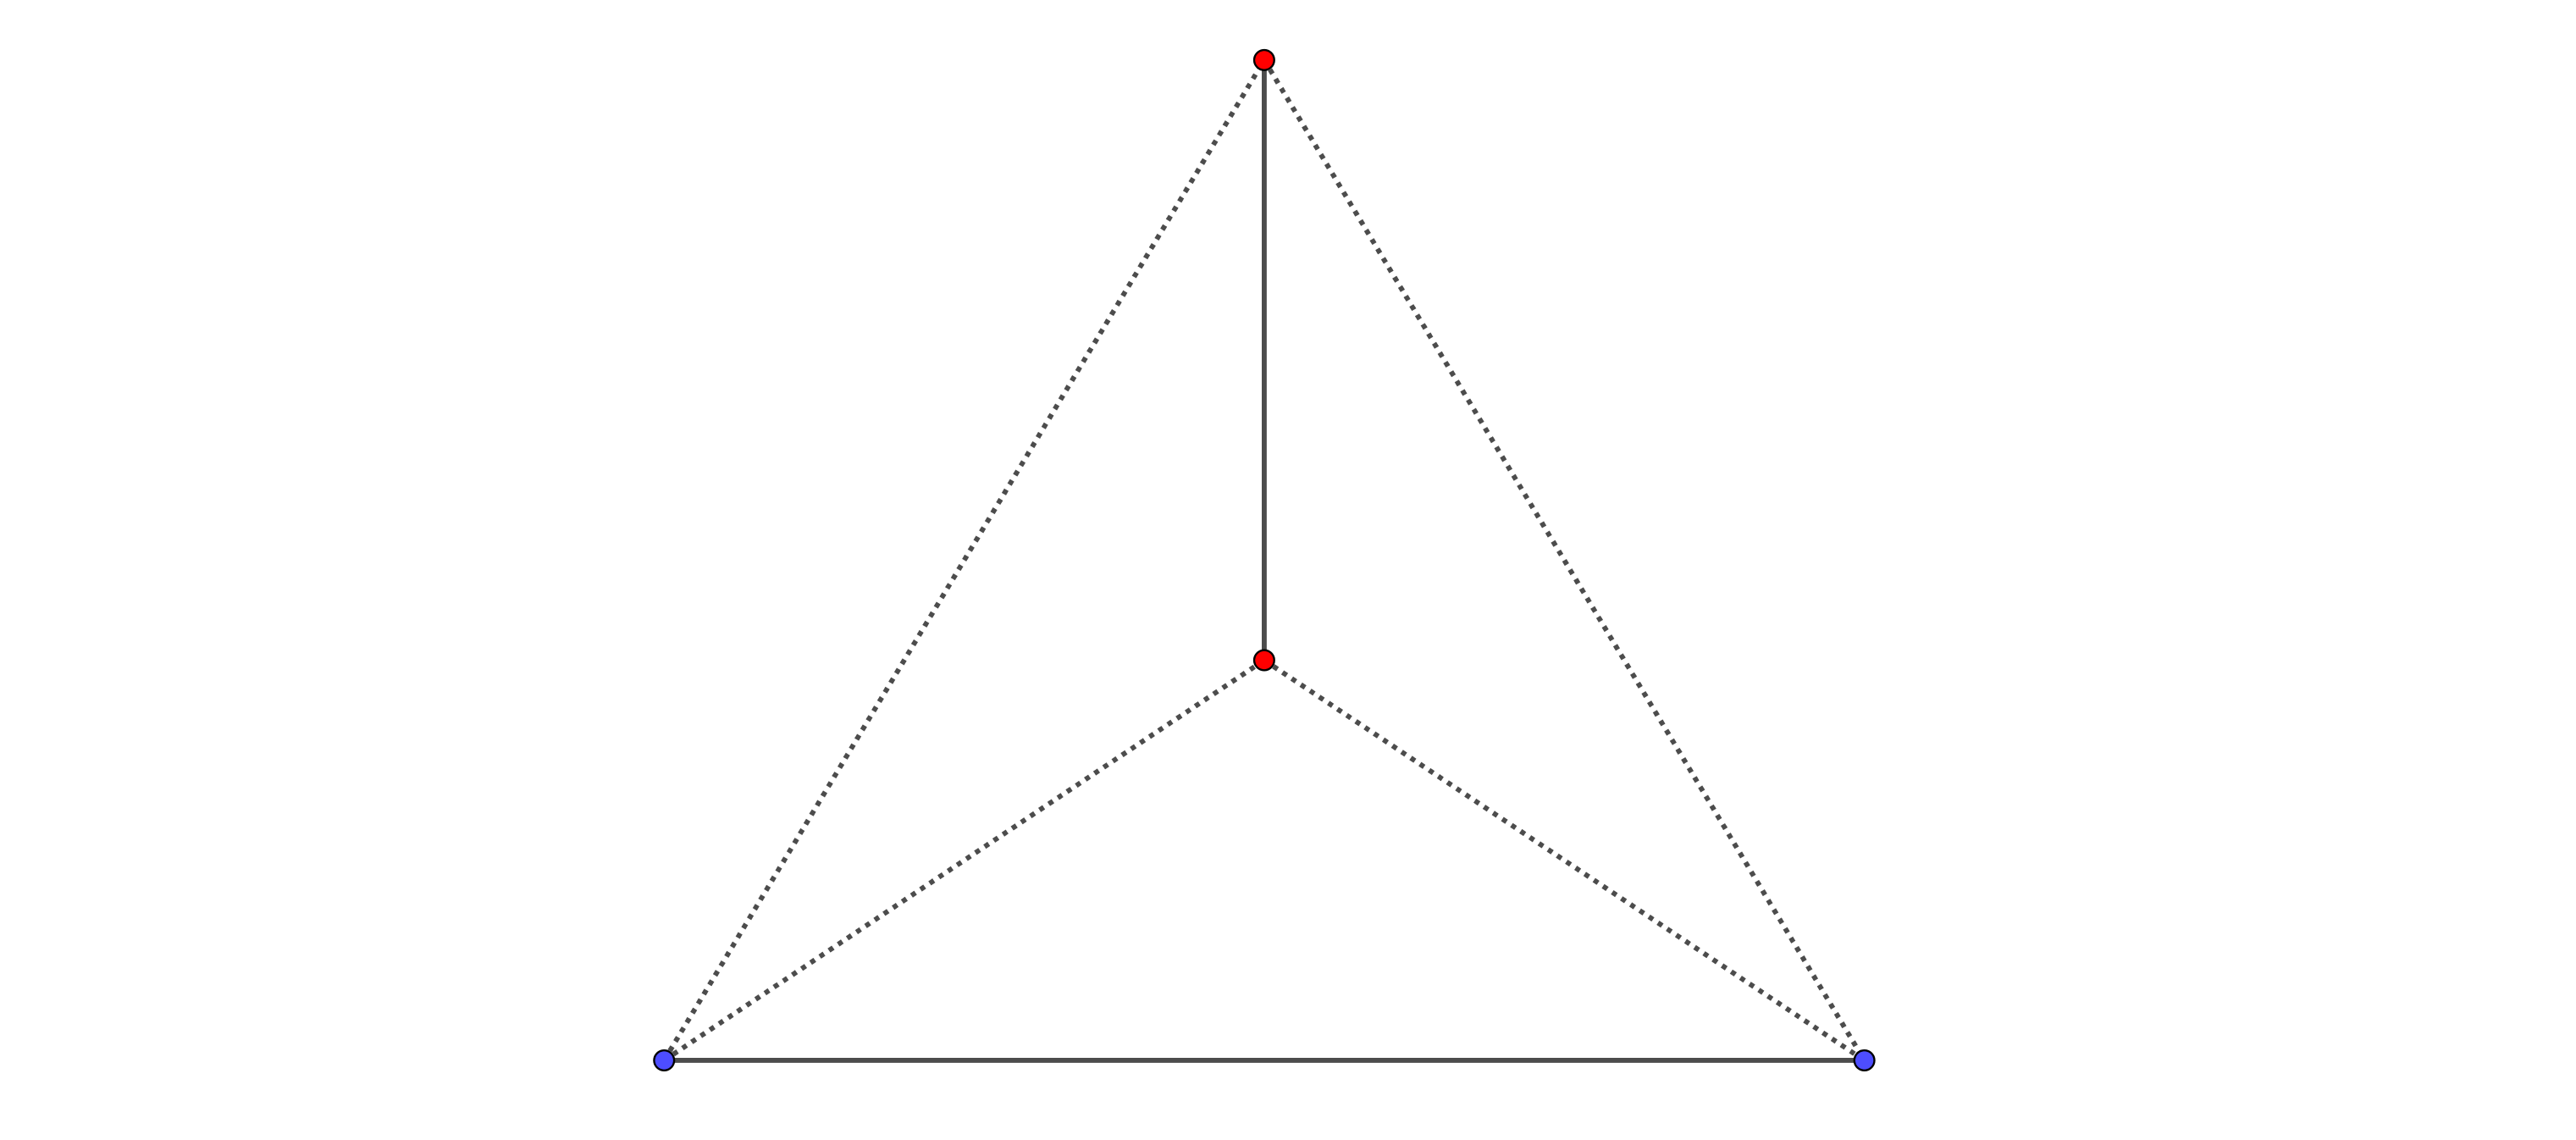
\includegraphics[width=\textwidth]{Tokunaga-3}
\end{figure}
\end{frame}
\begin{frame}
\begin{figure}[h]
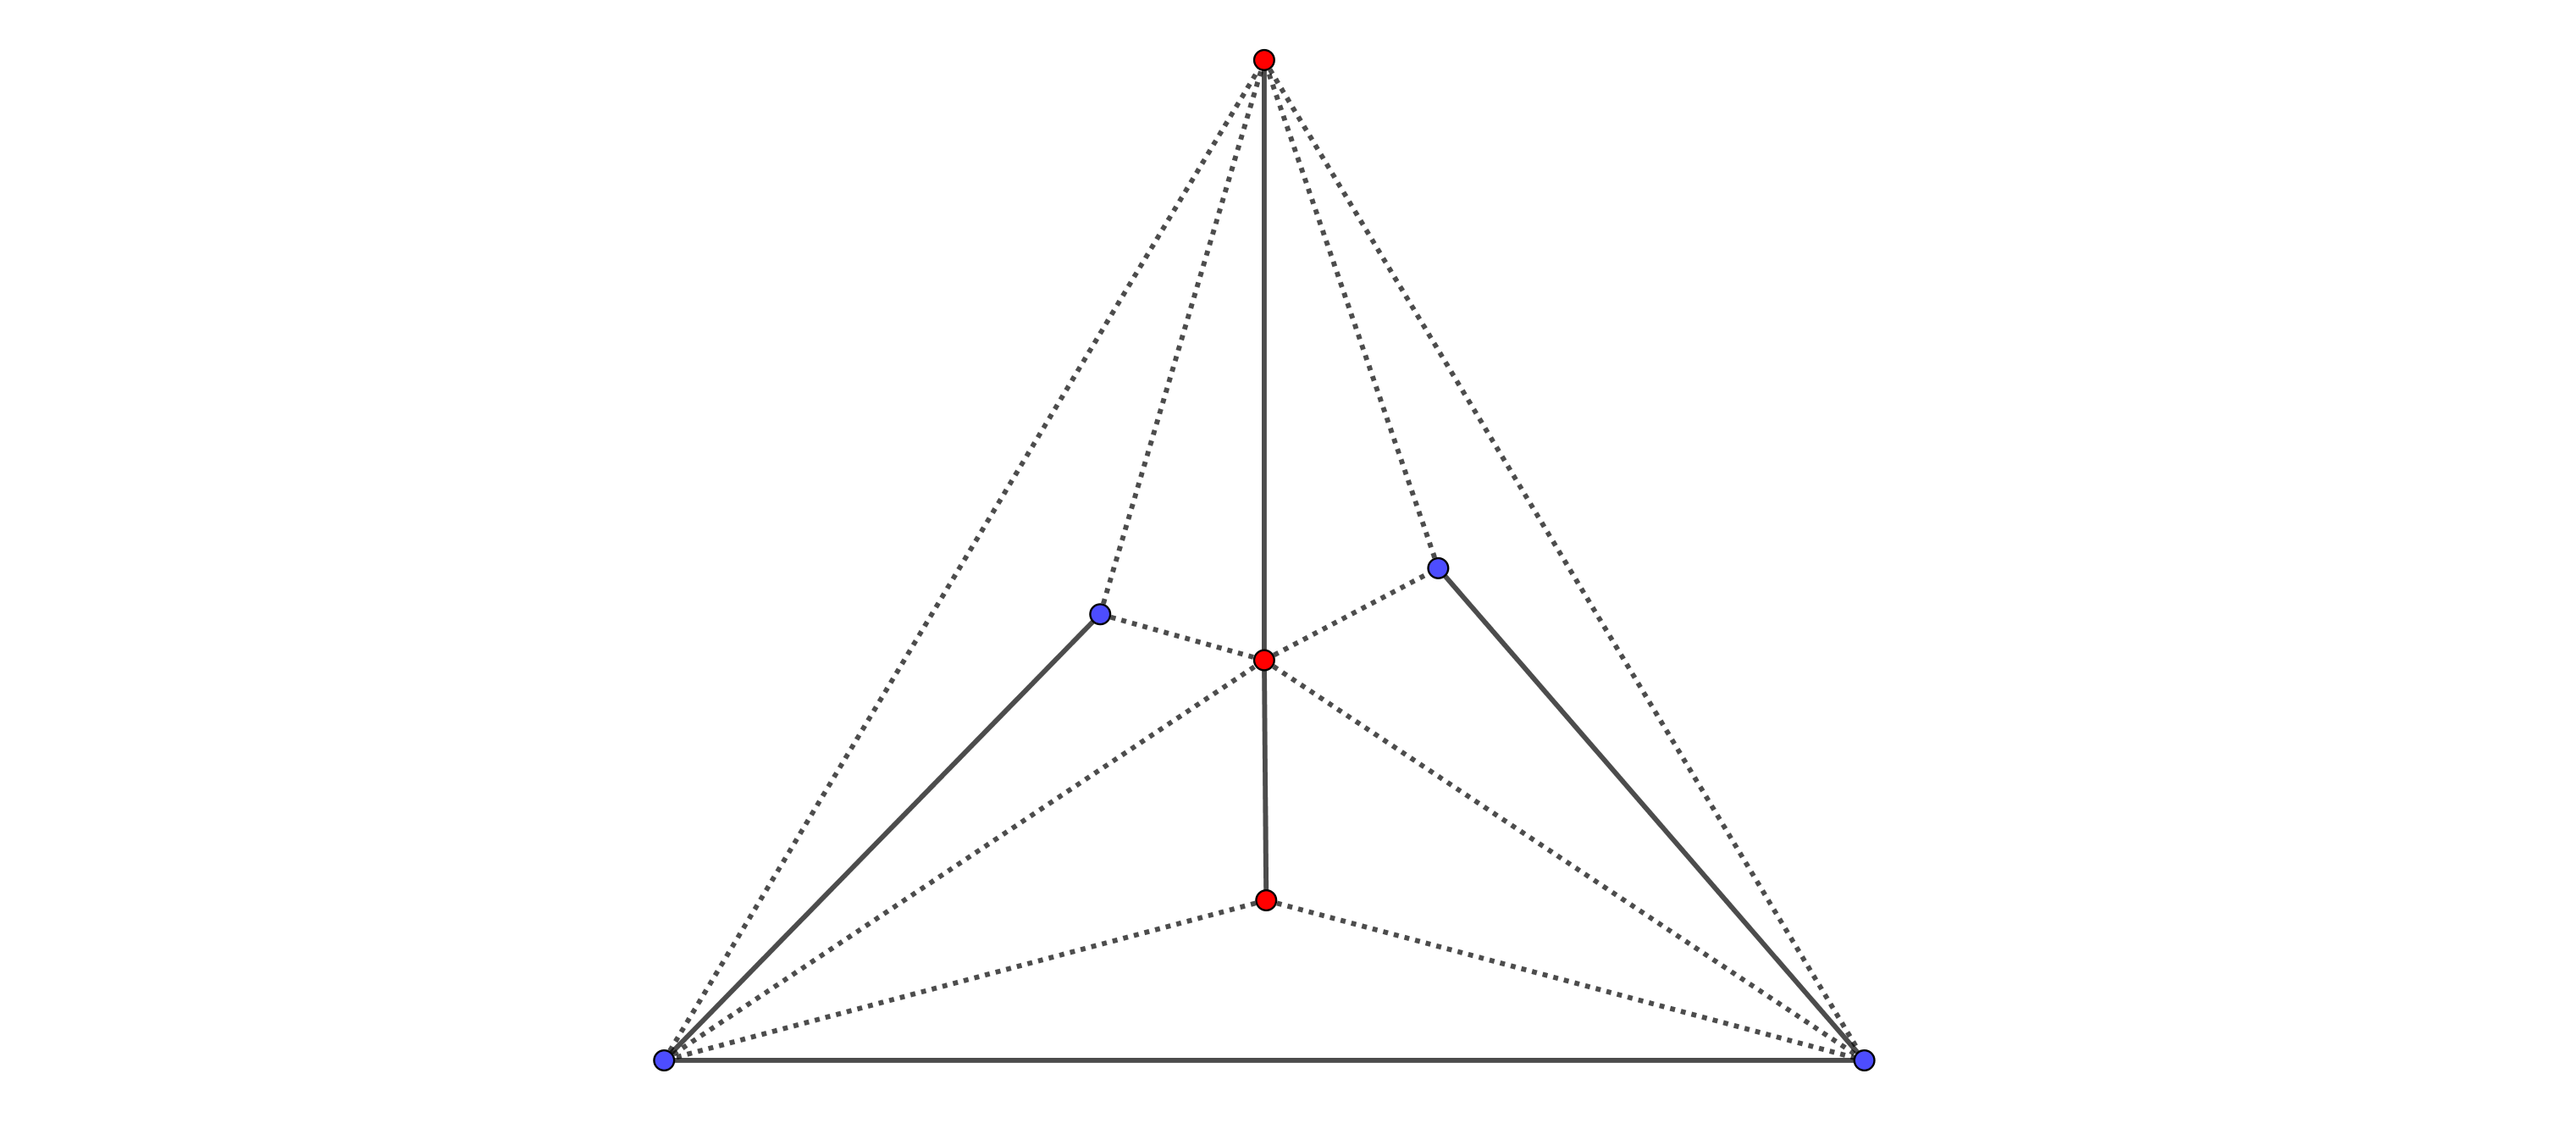
\includegraphics[width=\textwidth]{Tokunaga-4}
\end{figure}
\end{frame}
\begin{frame}
\begin{figure}[h]
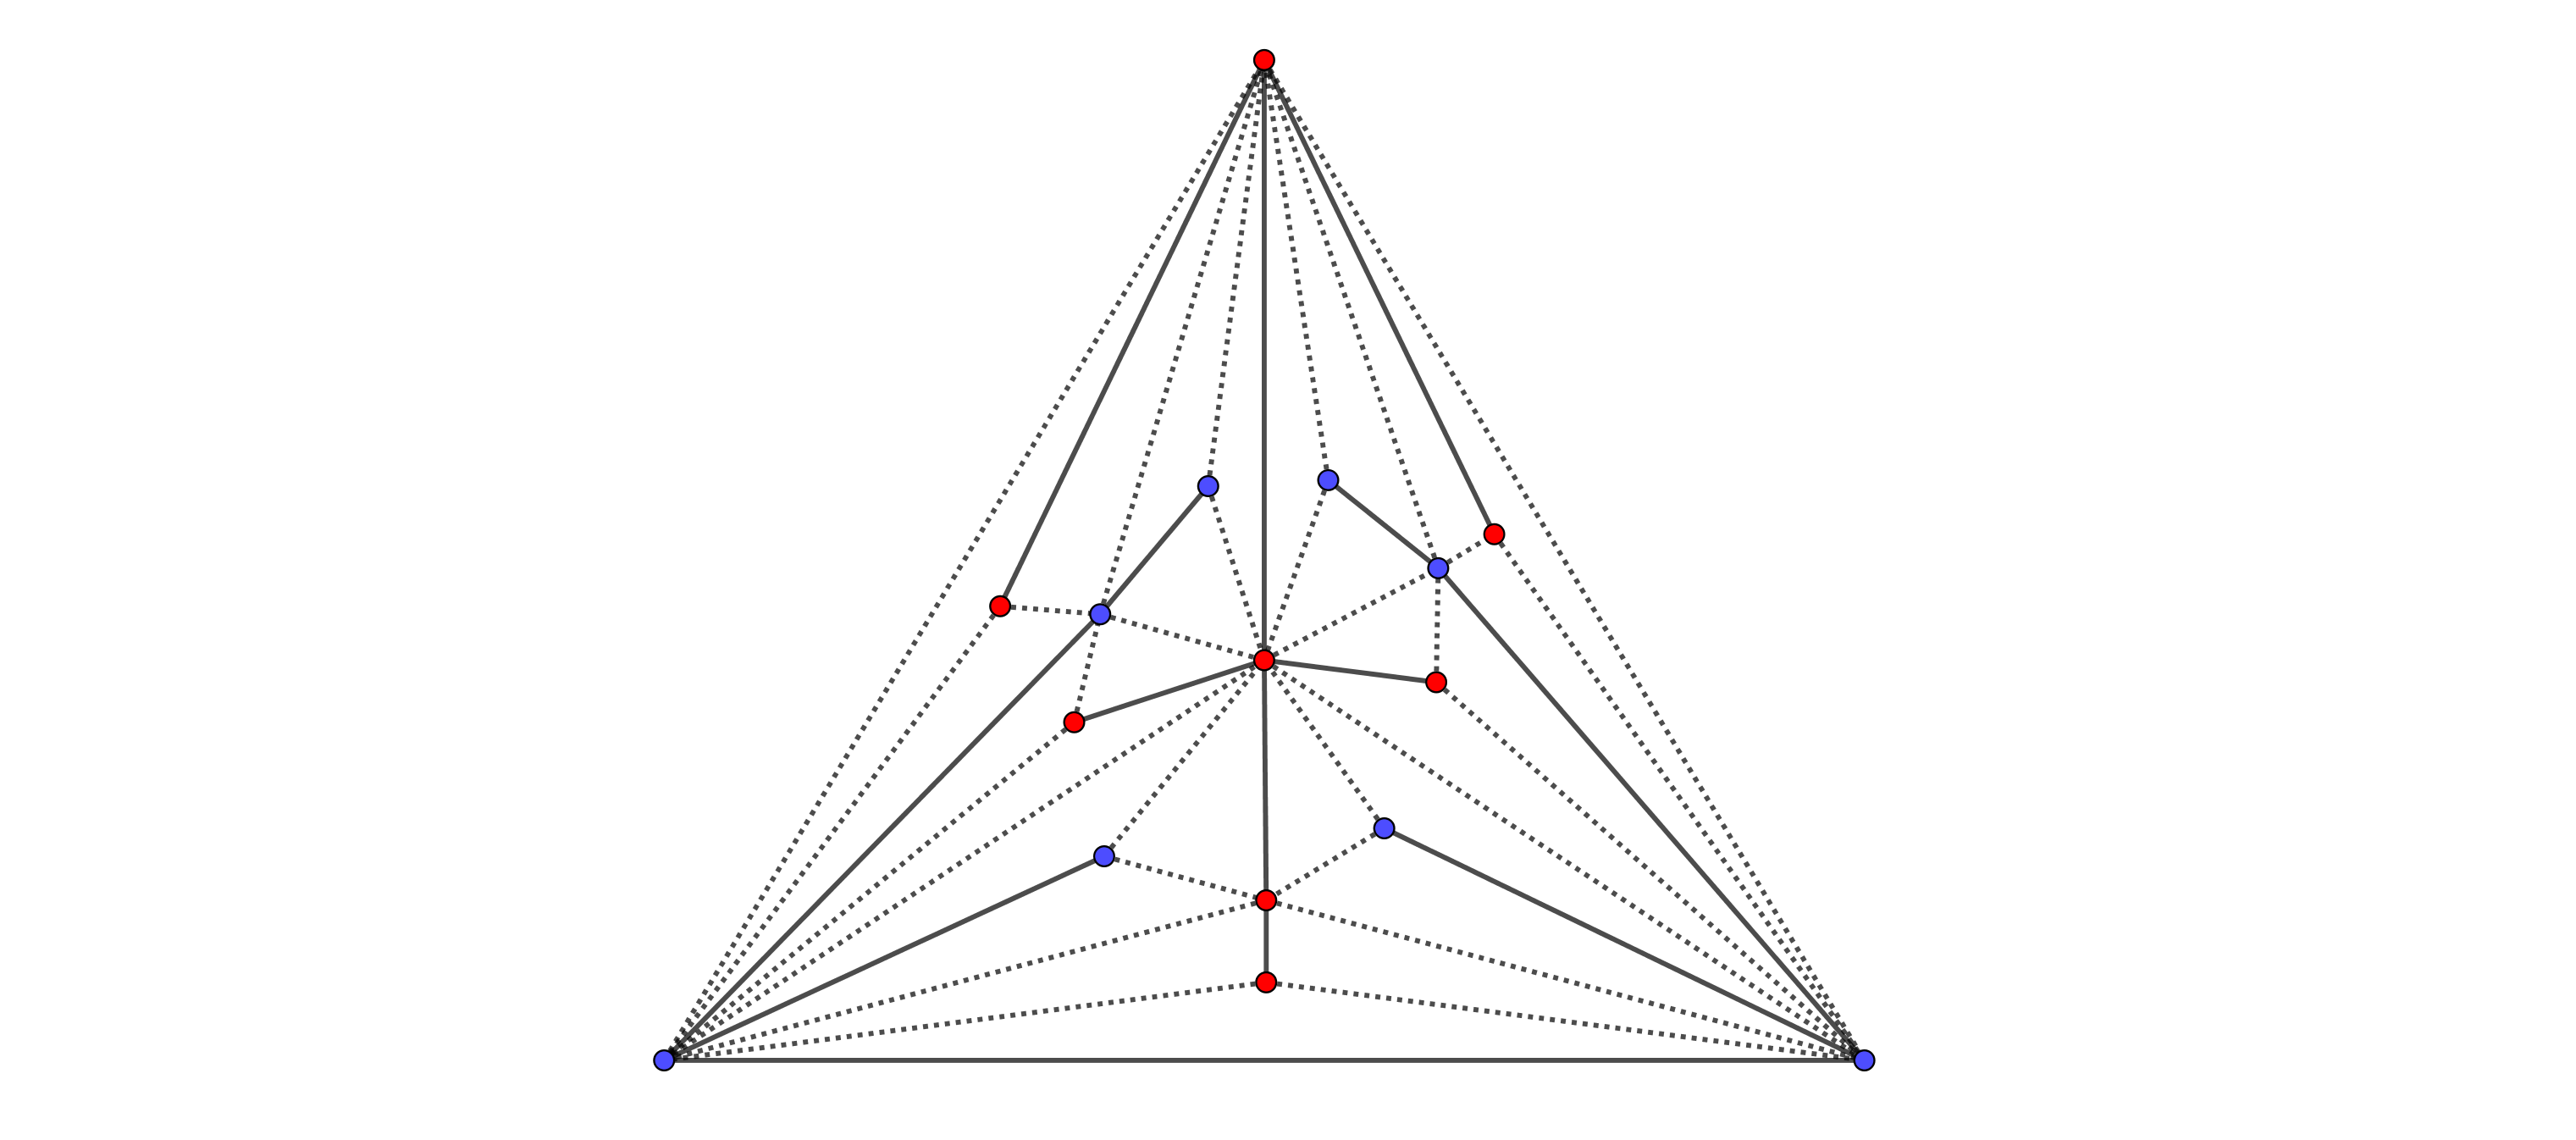
\includegraphics[width=\textwidth]{Tokunaga-5}
\end{figure}
\end{frame}
\begin{frame}
\begin{figure}[h]
\includegraphics[width=\textwidth]{Ejemplo-X-arbol}
\end{figure}
\end{frame}
\begin{frame}
\begin{figure}[h]
\includegraphics[width=\textwidth]{Ejemplo-X-arbol-2}
\end{figure}
\end{frame}
\begin{frame}
\begin{figure}[h]
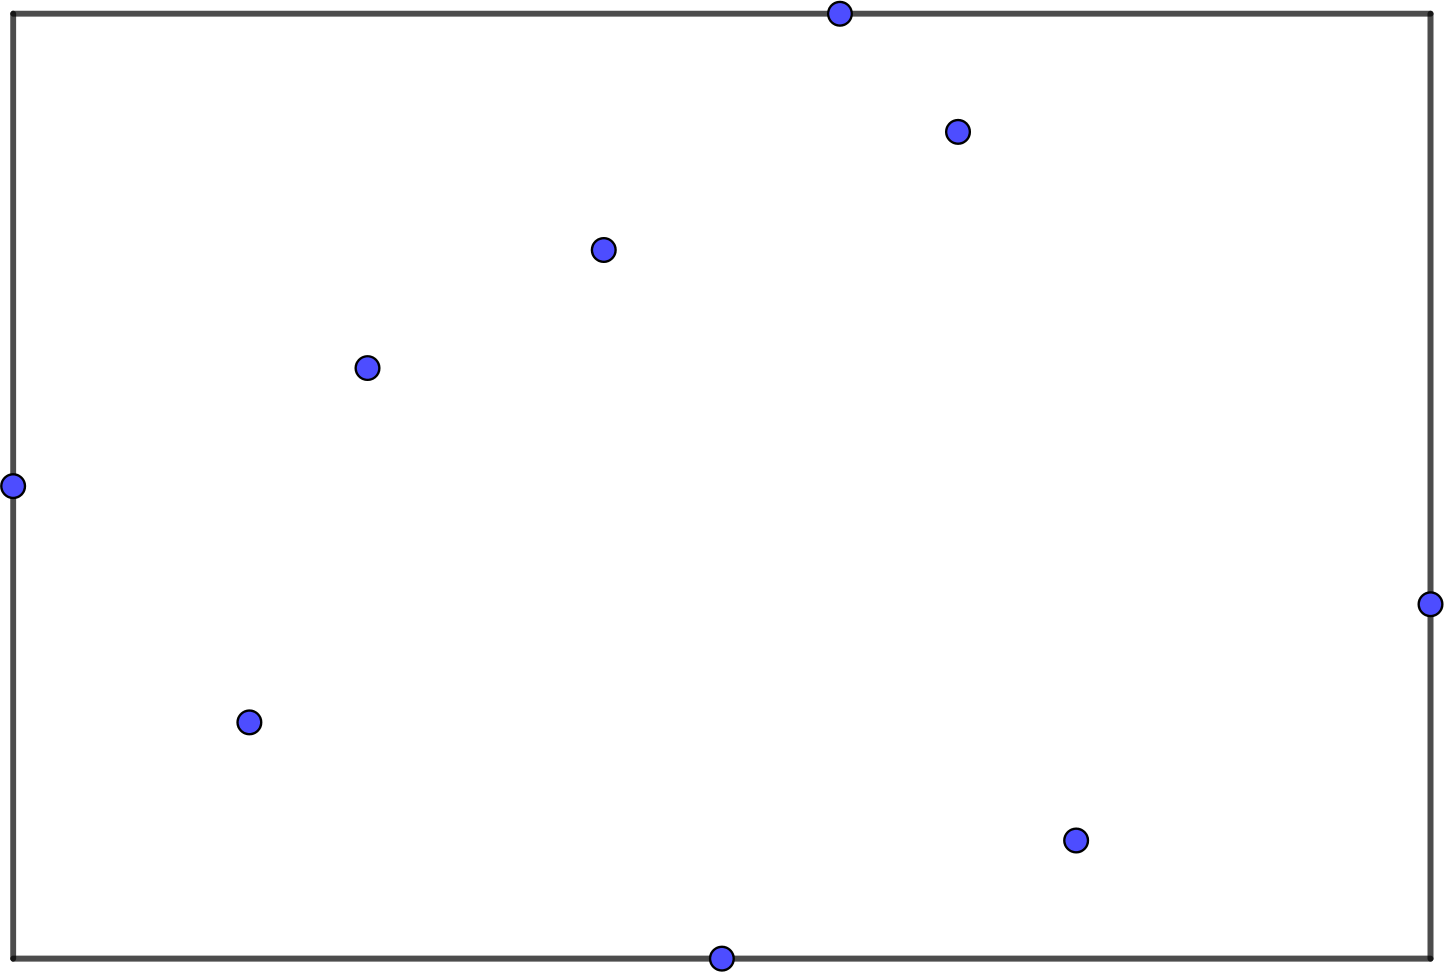
\includegraphics[width=\textwidth]{Ejemplo-rect-S}
\end{figure}
\end{frame}
\begin{frame}
\begin{figure}[h]
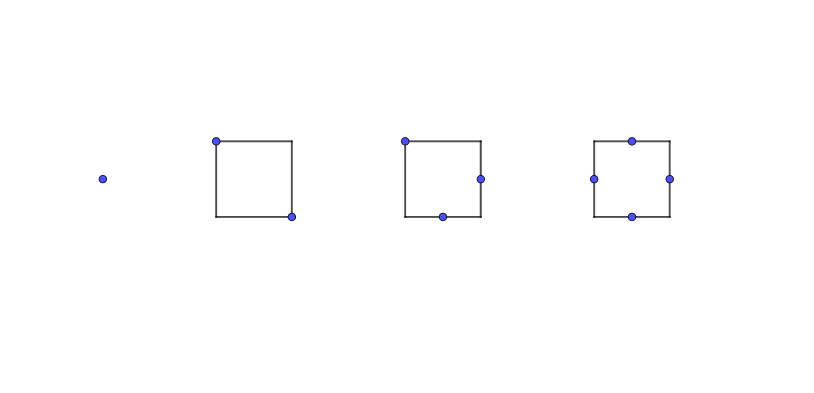
\includegraphics[width=\textwidth]{Cantidad-en-rect-S}
\end{figure}
\end{frame}
\begin{frame}
\begin{figure}[h]
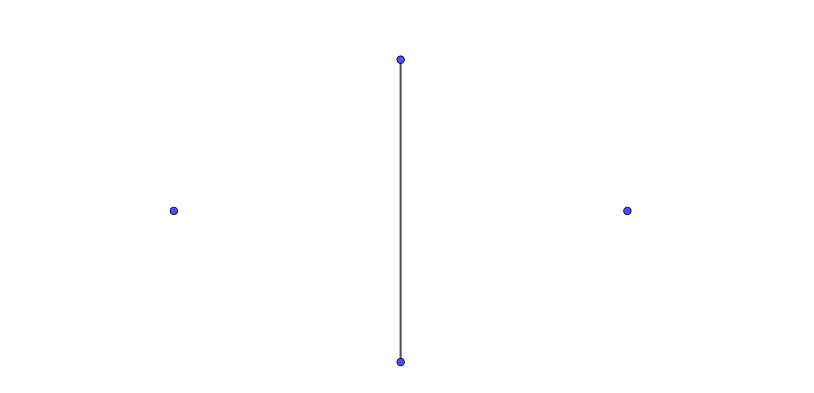
\includegraphics[width=\textwidth]{Arbol-imposible-sin-cruces}
\end{figure}
\end{frame}
\begin{frame}
\begin{figure}[h]
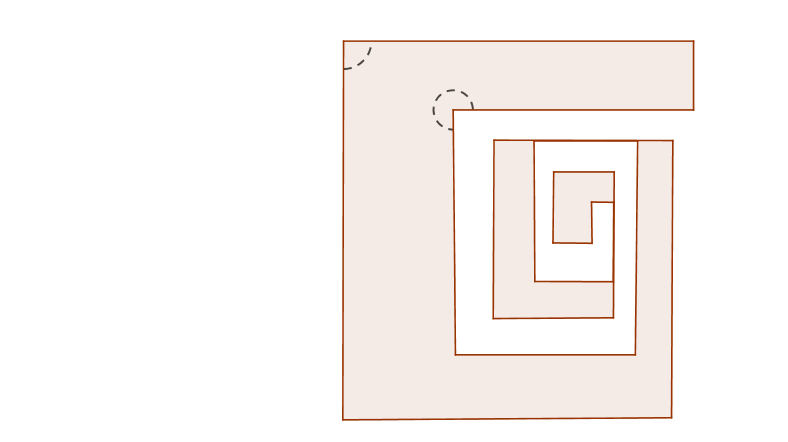
\includegraphics[width=\textwidth]{Poligono-espiral}
\end{figure}
\end{frame}


\end{document}